\documentclass[11pt,a4paper]{article}

\usepackage[utf8]{inputenc}
\usepackage[T1]{fontenc}
\usepackage[english]{babel}
\usepackage{mathptmx}
\usepackage{microtype}
\usepackage[margin=2.5cm]{geometry}
\usepackage{amsmath,amssymb,amsthm}
\usepackage{graphicx}
\usepackage{booktabs}
\usepackage{array}
\usepackage{xcolor}
\usepackage{listings}
\usepackage{enumitem}
\usepackage{tikz}
\usetikzlibrary{decorations.pathreplacing}
\usepackage[hidelinks,pdfauthor={Independent author},pdftitle={Births outside the light cone},pdfcreator={},pdfproducer={}]{hyperref}

\newtheorem{theoremL}{Theorem}
\renewcommand{\thetheoremL}{\Alph{theoremL}}
\newtheorem{proposition}{Proposition}
\newtheorem{lemma}{Lemma}
\newtheorem{corollary}{Corollary}
\newtheorem{conjecture}{Conjecture}
\theoremstyle{definition}
\newtheorem{definition}{Definition}
\newtheorem{estimate}{Estimate}
\newtheorem{example}{Example}
\theoremstyle{remark}
\newtheorem{remark}{Remark}

\newcommand{\Inf}{\mathrm{Inf}}
\newcommand{\Abar}{\bar A}
\newcommand{\E}{\mathbb{E}}
\newcommand{\Srec}{S_2^{\mathrm{ann}}}
\newcommand{\dket}[1]{|#1\rangle\!\rangle}
\newcommand{\dbra}[1]{\langle\!\langle #1|}
\newcommand{\dd}{\mathrm{d}}
\newcommand{\repo}{\url{https://github.com/GofKingnose/births-outside-the-light-cone}}
\renewcommand{\epsilon}{\varepsilon}
\setlength{\emergencystretch}{3em}

\lstdefinelanguage{Coq}{
  keywords={Require,Import,Open,Scope,Lemma,Theorem,Corollary,Proof,Qed,forall,let,in,intros,unfold,assert,by,field,assumption,split,intro,nra,lra,rewrite,apply,destruct,ring,Fixpoint,Definition,Inductive,match,with,end,if,then,else,exact,induction,as,pose,proof,lia,Section,Variable,Variables,Hypothesis,End},
  comment=[n]{(*}{*)}, morestring=[b]"}
\lstset{language=Coq,basicstyle=\ttfamily\footnotesize,keywordstyle=\bfseries,
  commentstyle=\itshape\color{gray},columns=fullflexible,breaklines=true,frame=single,
  literate={Ā}{{$\bar A$}}1 {⊆}{{$\subseteq$}}1 {≤}{{$\leq$}}1}

\title{\textbf{Births outside the light cone}\\[5pt]
\large Entropy deficit in a growing quantum register:\\
causal bounds, optimality, and exact results for random circuits}
\author{Independent author\thanks{Contact: \texttt{github.kabob469@passmail.com}. Code, data, Coq proofs and the \LaTeX{} source: \repo{} (release v1.0.0). \textbf{AI-use statement:} this work was produced by an AI system (Claude, Anthropic) in an extended interactive session directed by the author, who posed the research questions and made editorial decisions. The derivations, proofs, Coq formalisation, code, numerical experiments and text were generated by the AI system. The author has not independently verified the mathematical content, and the work has so far been checked only by automated reviewers. Please report errors through the repository's issue tracker.}}
\date{October 2026}

\begin{document}
\maketitle

\begin{abstract}
We study a quantum register whose Hilbert space grows: fresh qudits are born in a pure state, uncorrelated with the rest, and the register is scrambled by local dynamics. The observable is the deficit $G(A)=\log q\,\min(|A|,|\Abar|)-S(A)$ between the maximal and the actual entropy of a region. A velocity criterion in the spirit of Frautschi (relaxation versus expansion) predicts that the deficit closes when scrambling is fast enough; simulations refute it. We show that the controlling variable is causal, not kinetic.
(i)~For every unitary circuit, on any graph and with arbitrary births, $S(A)\le\log q\,|\Abar\cap\Inf(A)|$, where $\Inf(A)$ collects the qudits whose world line meets the causal past of $A$ (Theorem~A); a Lieb--Robinson version holds for local Hamiltonians (Theorem~B).
(ii)~For an isotropic front $R\propto t^\alpha$, the deficit is extensive for every local dynamics if $\alpha\ge1$, and can be made sub-extensive if $\alpha<1$ (Theorem~C); in one dimension the causal bound is attained.
(iii)~For gates drawn from a 2-design, the averaged purity of a prefix reduces \emph{exactly} to the walk of a single domain wall absorbed by the line of births. This yields $\E[G]=\Theta(m^{2-1/\alpha})$ for $\frac12<\alpha<1$ (Theorem~D) and, for one birth every $k$ layers, the exact annealed Rényi-2 density $\theta_k$ with $\frac{2q}{q^2+1}\cosh\theta_k=e^{-\theta_k/k}$ (Theorem~E).
(iv)~Stabilizer simulations up to $6400$ qubits and Haar state-vector simulations up to $22$ qubits agree with these statements; predictions were written before the computations, and the ones that failed are reported.
The deficit is robust to the choice of birth state and to local correlations with the past. In a free lattice field with a vacuum, however, uncorrelated births cost an energy of the order of the cutoff, so the cosmological reading of these results remains a constrained analogy.
\end{abstract}

\tableofcontents
%======================================================================
\section{Introduction}
%======================================================================

\paragraph{The question.} Consider a quantum register that grows. New degrees of freedom are born in a pure state, uncorrelated with what already exists, and the whole register is scrambled by local unitary dynamics. Scrambling drives the entropy of a region towards its maximum; births keep adding degrees of freedom whose entanglement with the rest starts at zero. Does the register catch up with its maximal entropy if scrambling is fast enough? If not, what controls the deficit?

\paragraph{Why it matters.} Growing registers appear in two settings. In quantum processors, fresh ancillas enter a computation mid-circuit; entanglement in the presence of resets and fresh qudits is an active topic \cite{PSQ2020,Yokoyama2026}. In cosmology, a fixed ultraviolet cutoff in an expanding universe seems to require a growing Hilbert space \cite{Jacobson1999}, and several toy models of this kind have been proposed: circuits in which unentangled ancillas are progressively entangled \cite{Bao2017}, isometric rather than unitary evolution \cite{CotlerStrominger2022}, and de Sitter tensor networks \cite{BaoDS2017,Cao2023}. Layzer \cite{Layzer1975} and Frautschi \cite{Frautschi1982} noted long ago that in an expanding universe the maximal entropy accessible to a causal region can grow faster than the actual entropy, and that a system ``falls out of equilibrium if its relaxation time exceeds the expansion time''. This is a \emph{velocity} criterion: it predicts a return to equilibrium as soon as relaxation is fast enough.

\paragraph{A refuted prediction.} This work started from a prediction written before any computation: the Frautschi criterion transposed to circuits, according to which the deficit closes when $k\,v_E\gtrsim\frac12$, where $k$ is the number of scrambling layers per birth and $v_E$ the entanglement velocity. Simulations refuted it: the deficit stays extensive for every $k$ tested, from $1$ to $32$ (Section~\ref{sec:num-edge}). This failure is the origin of the results below.

\paragraph{Answer.} The deficit does not depend primarily on the scrambling rate. It depends on the fraction of degrees of freedom that are born \emph{outside the causal past} of the region considered. Table~\ref{tab:glance} summarises the results and their status.

\begin{table}[h]
\centering\small\setlength{\tabcolsep}{4pt}
\begin{tabular}{p{3.2cm}p{8.3cm}p{2.9cm}}
\toprule
result & statement & status\\
\midrule
Theorem~A (Sec.~\ref{sec:A}) & $S(A)\le\log q\,|\Abar\cap\Inf(A)|$ for every unitary circuit, any graph, any births & proven; combinatorial core in Coq\\
Theorem~B (Sec.~\ref{sec:A}) & Lieb--Robinson version for local Hamiltonians on a fixed graph & proven from a cited bound\\
Proposition~\ref{prop:births} & any pure birth state; mixed births; births correlated with the past & proven\\
Theorem~C (Sec.~\ref{sec:geo}) & front $R\propto t^\alpha$: extensive deficit for every dynamics iff $\alpha\ge1$ & proven (isotropic fronts)\\
Proposition~A1 (Sec.~\ref{sec:A1}) & in 1D the causal bound is attained & proven; arithmetic in Coq\\
Theorem~D (Sec.~\ref{sec:walls}) & 2-design gates: $\E[G]$ is set by the births of two recent windows; $\Theta(m^{2-1/\alpha})$ for $\frac12<\alpha<1$ & proven\\
Theorem~E (Sec.~\ref{sec:walls}) & exact annealed Rényi-2 density $\theta_k$ at $\alpha=1$; proven bracket on $\E[G]/N$ & proven\\
Proposition~\ref{prop:obstruction} (Sec.~\ref{sec:dimsup}) & no single-wall reduction in 2D; membrane conjecture & proven obstruction; conjecture\\
Numerics (Sec.~\ref{sec:num}) & stabilizer simulations to $6400$ qubits, Haar to $22$ qubits & pre-registered\\
Section~\ref{sec:energy} & in a free lattice field, uncorrelated births cost energy $\sim0.07$ of the cutoff & numerical, exact Gaussian\\
\bottomrule
\end{tabular}
\caption{Results at a glance. The full status of each statement, including which parts are formally verified, is given in Table~\ref{tab:status}.}
\label{tab:glance}
\end{table}

\paragraph{What the paper does not do.} The register has no gravity, no conserved energy and no Friedmann equation. The results do not derive an arrow of time from nothing: they derive it from a \emph{birth condition}, namely that a new degree of freedom is not correlated at long distance with what already exists. Section~\ref{sec:energy} shows that, as soon as there is a vacuum and an energy, this condition costs an energy of the order of the cutoff per degree of freedom, in agreement with an objection of Foster and Jacobson \cite{FosterJacobson2004}, while the energetically admissible birth is correlated with the past and carries no deficit of its own. The cosmological readings of Section~\ref{sec:discussion} are therefore analogies; the natural domain of the results is that of growing quantum registers.

\paragraph{Outline.} Section~\ref{sec:setting} sets up the model. Section~\ref{sec:A} proves the causal bound and examines general births. Section~\ref{sec:geo} turns the bound into a geometric dichotomy. Section~\ref{sec:A1} proves optimality in one dimension. Section~\ref{sec:walls} derives the exact single-wall model for 2-design circuits and Theorems~D and~E; Section~\ref{sec:dimsup} explains why it does not extend to two dimensions. Section~\ref{sec:num} reports the numerical tests, Section~\ref{sec:energy} the energetic cost of the birth condition, and Section~\ref{sec:discussion} discusses the status of each statement, prior work and limitations. The appendices contain the longer proofs, the Coq formalisation and a reproducibility guide.

%======================================================================
\section{Setting}\label{sec:setting}
%======================================================================

\subsection{Register, births, circuits}

A \emph{degree of freedom} (site) $x$ is a qudit of dimension $q\ge2$. It is born at time $t_x\ge0$ in the state $|0\rangle$, in a product with everything else; this is the precise meaning of ``uncorrelated''. The sites present at $t=0$ are in a pure product state. A birth is thus the isometry $|\psi\rangle\mapsto|\psi\rangle\otimes|0\rangle_x$: the global state stays pure and the total entropy stays zero. The dynamics is a circuit of \emph{unitary} gates $g_1,\dots,g_M$ applied at times $\tau_1\le\dots\le\tau_M$. Each gate acts on a finite support $\mathrm{supp}(g_j)$ of sites already born ($t_x\le\tau_j$), with arbitrary arity. We write $\Lambda_T$ for the set of sites born by the final time $T$, $N=|\Lambda_T|$, and $A\subset\Lambda_T$ for a region. The observable is
\begin{equation}\label{eq:G}
G(A)=\log q\,\min(|A|,|\Abar|)-S(A)\ \ge0 .
\end{equation}
Since the global state is pure, $S(A)=S(\Abar)$ and the mutual information is $I(A{:}\Abar)=2S(A)$: any growth of $S(A)$ is a growth of correlations between $A$ and $\Abar$. For a Haar-random state, $G$ equals the Page correction, $O(1)$ \cite{Page1993}. An \emph{extensive} deficit, $G\ge cN$ with $c>0$, therefore signals a durable arrow.

\begin{lemma}[birth = idle qudit]\label{lem:idle}
The final state is the same as if all sites existed from $t=0$ in the state $|0\rangle$, with no gate acting on $x$ before $t_x$.
\end{lemma}
\begin{proof}
Inserting $|0\rangle$ at time $t_x$, or keeping it in reserve from $t=0$ without touching it, produces the same vector.
\end{proof}

Growth thus becomes a \emph{progressive switching-on of couplings} on a fixed set, starting from a pure product state. All the low-entropy structure lies in this birth hypothesis; Proposition~\ref{prop:births} examines what survives when it is weakened.

\subsection{Causal past}

\begin{definition}[backward sweep]
Set $C_M=A$ and, for $j=M,\dots,1$, $C_{j-1}=C_j\cup\mathrm{supp}(g_j)$ if $\mathrm{supp}(g_j)\cap C_j\neq\emptyset$ (we then say that gate $g_j$ is \emph{in the cone}), and $C_{j-1}=C_j$ otherwise. We write $\Inf(A)=C_0$: the set of sites whose world line meets the causal past of $A$.
\end{definition}

This cone is \emph{strict}: it depends on the structure of the circuit (which gate acts on which sites, and when), not on the gates themselves. The sweep is implemented in \texttt{code/tableau.py} (function \texttt{infected}), and the single-wall recursion of Section~\ref{sec:walls} in \texttt{code/domain\_wall.py} (function \texttt{logZ\_wall}).

\begin{example}\label{ex:sweep}
Four sites $0,1,2,3$, region $A=\{0,1\}$, and three gates in temporal order: $g_1$ on $(1,2)$, then $g_2$ on $(2,3)$, then $g_3$ on $(0,1)$. Going backwards: $g_3$ touches $A$, so $C=\{0,1\}$; $g_2$ does not touch $\{0,1\}$ and is outside the cone; $g_1$ touches site $1$, so $C=\{0,1,2\}$. Hence $\Inf(A)=\{0,1,2\}$ and $|\Abar\cap\Inf(A)|=1$. Theorem~A below then gives $S(A)\le\log q$, although $\min(|A|,|\Abar|)=2$: site $3$, whether born at $t=0$ or just before $g_2$, never interacts with anything that later reaches $A$, so $G(A)\ge\log q$.
\end{example}

\subsection{Reference architectures}\label{sec:archi}

\emph{Dimension 1, edge growth}: a chain with two-qudit gates in a brickwork pattern; layer $L$ acts on the pairs $(x,x+1)$ with $x\equiv L\pmod2$. A site is born at the right edge every $k$ layers, just before layer $L$ if $L\equiv0\pmod k$. The cone advances by one site per layer. \emph{Dimension 1, insertion}: sites are inserted at uniformly random positions, following a law $N(t)$. \emph{Dimension 2}: a square lattice cut by a vertical line. A round consists of four sub-layers (horizontal even and odd, vertical even and odd); the causal speed normal to the cut is $v=2$ sites per round. Births follow a circular front, a constant global rate, or the Eden model.

%======================================================================
\section{The causal bound}\label{sec:A}
%======================================================================

\begin{theoremL}\label{thm:A}
For every circuit of unitary gates and every region $A\subset\Lambda_T$,
\begin{equation}\label{eq:A}
S(A)\le\log q\,\big|\Abar\cap\Inf(A)\big| ,
\end{equation}
and therefore, since $S(A)=S(\Abar)$,
\begin{equation}\label{eq:Agap}
G(A)\ge\log q\Big[\min(|A|,|\Abar|)-\min\big(|\Abar\cap\Inf(A)|,\,|A\cap\Inf(\Abar)|\big)\Big].
\end{equation}
\end{theoremL}

\begin{proof}
\emph{(1) Idle sites.} By Lemma~\ref{lem:idle}, the initial state is $|\Psi_0\rangle=\bigotimes_x|0\rangle_x$ on all sites.
\emph{(2) Splitting.} The backward sweep splits the gates into two ordered subsequences, $\mathcal C_{\rm in}$ (in the cone) and $\mathcal C_{\rm out}$ (outside the cone). Four combinatorial facts follow; they are proven in Coq (Appendix~\ref{app:coq}):
(a)~$A\subseteq\Inf(A)$;
(b)~every gate of $\mathcal C_{\rm in}$ acts inside $\Inf(A)$;
(c)~no gate of $\mathcal C_{\rm out}$ acts on $A$;
(d)~for every semantics in which gates with disjoint supports commute, applying the circuit is the same as applying $\mathcal C_{\rm in}$ and then $\mathcal C_{\rm out}$. Point~(d) holds because a gate outside the cone is disjoint from every cone gate that follows it.
\emph{(3) Purity.} Let $C=\Inf(A)$. By (b), $\mathcal C_{\rm in}|\Psi_0\rangle=|\varphi\rangle_C\otimes|0\cdots0\rangle_{\Lambda\setminus C}$ with $|\varphi\rangle_C$ pure, because the gates are unitary.
\emph{(4) Conclusion.} By (d) and (c), the final state is $W\,\mathcal C_{\rm in}|\Psi_0\rangle$, where $W$ is a unitary on $\Lambda\setminus A$. Hence $\rho_A=\mathrm{Tr}_{C\setminus A}|\varphi\rangle\langle\varphi|$. Since $|\varphi\rangle$ is pure on $C=A\sqcup(C\setminus A)$, $S(A)=S(C\setminus A)\le\log q\,|\Abar\cap C|$.
\end{proof}

\begin{remark}[the quantum facts used]\label{rem:quantumfacts}
Besides the combinatorial facts (a)--(d), the proof uses only four facts of finite-dimensional quantum mechanics: (i)~a unitary acting on $C$ maps a pure product state to a state that is pure on $C$; (ii)~for a pure state on $A\sqcup B$, $S(A)=S(B)$ (Schmidt decomposition); (iii)~$S(B)\le\log\dim\mathcal H_B=|B|\log q$; (iv)~a unitary acting on the complement of $A$ does not change $\rho_A$ (invariance of the partial trace). Formalising them in Coq would require a library of finite-dimensional linear algebra and quantum states; this is a project in itself and is not done here.
\end{remark}

\begin{remark}[scope]
The theorem assumes nothing about the unitary gates (Haar, Clifford or deterministic) or about the graph, which may change in time; it therefore covers the insertion of sites between existing ones. It is a special case of the Schmidt-rank bound across a cut of the tensor network, in which a fresh site is a leg of dimension~$1$ \cite{Hayden2016,NRVH2017}, and it belongs to the family of light-cone bounds on the generation of correlations and entanglement \cite{BHV2006,EisertOsborne2006,Bravyi2007}. Its only specific content is the application to growth.
\end{remark}

\begin{corollary}[geometric form]\label{cor:geo}
Let $\mathrm d_\perp$ be a distance, for instance the distance normal to the cut, for which every gate has a support of diameter at most~$1$. Let $n_\perp(t,T)$ be the number of layers in $[t,T]$ that contain at least one gate of $\mathrm d_\perp$-diameter~$1$. Then $\Abar\cap\Inf(A)\subseteq\{x\in\Abar:\mathrm d_\perp(x,A)\le n_\perp(t_x,T)\}$. In particular, if $|\Abar|\le|A|$,
\begin{equation}\label{eq:geo}
G(A)\ge\log q\;\#\big\{x\in\Abar:\ \mathrm d_\perp(x,A)>n_\perp(t_x,T)\big\}.
\end{equation}
For periodic layers, $n_\perp(t,T)\le v(T-t)+c_0$, with $c_0=1$ in 1D and $c_0=2$ for the 2D pattern of Section~\ref{sec:archi}.
\end{corollary}
\begin{proof}
Going backwards in time, only these layers can move the edge of the cone away from $A$, by at most one unit each, and a site $x$ can only be reached by a gate applied after $t_x$.
\end{proof}

\subsection{General births}\label{sec:births}

The birth hypothesis of Section~\ref{sec:setting} can be weakened in three directions.

\begin{proposition}[robustness of the birth condition]\label{prop:births}
\begin{enumerate}[label=(\alph*),leftmargin=*]
\item \emph{Any pure birth state.} If site $x$ is born in a fixed pure state $|\phi_x\rangle$, possibly different from site to site, Theorems~A to~E and Proposition~A1 hold unchanged.
\item \emph{Mixed births.} If site $x$ is born in a state $\rho_x$ of entropy $s_x$, correlated only with a system outside the register, then
\begin{equation}\label{eq:Amixed}
S(A)\le\log q\,|\Abar\cap\Inf(A)|+\sum_{x\in\Inf(A)}s_x .
\end{equation}
\item \emph{Births correlated with the past.} A birth correlated with the existing register is an isometry $V_x:\mathcal H_{P_x}\to\mathcal H_{P_x}\otimes\mathcal H_x$, where $P_x$ is a set of sites already born. It can be written as a birth in $|0\rangle_x$ followed by a unitary gate supported on $P_x\cup\{x\}$, and Theorem~A applies to the completed circuit. If $P_x$ lies entirely on one side of a cut and $x$ on the other, the birth increases $S(A)$ by at most $S(x)=\tfrac12 I(x{:}\text{past})$, evaluated just after the birth.
\end{enumerate}
\end{proposition}
\begin{proof}
(a)~The proof of Theorem~A only uses the purity and the product structure of the initial state. For Theorems~D and~E, Lemma~\ref{lem:fresh} holds for every normalised pure state, $\langle\!\langle\pi|(|\phi\rangle\langle\phi|)^{\otimes2}\rangle\!\rangle=\mathrm{Tr}\,\pi(|\phi\rangle\langle\phi|)^{\otimes2}=1$, so $Z_A$ is unchanged. Proposition~A1 is a bound on the cone together with a Clifford construction; it suffices to precede each birth by a local gate that maps $|\phi_x\rangle$ to $|0\rangle$.
(b)~Purify each $\rho_x$ with a reference system $R_x$ that no gate touches. By steps (2)--(3) of the proof of Theorem~A, the state of $C\cup R_C$, with $C=\Inf(A)$, is pure after $\mathcal C_{\rm in}$, and $\mathcal C_{\rm out}$ does not act on $A$. Hence $S(A)=S\big((C\setminus A)\cup R_C\big)\le\log q\,|C\setminus A|+\sum_{x\in C}S(R_x)$.
(c)~Every isometry $V_x$ can be written $U\,(\mathbb 1_{P_x}\otimes|0\rangle_x)$ with $U$ unitary on $P_x\cup\{x\}$. If $P_x\subseteq A$ and $x\in\Abar$, the Araki--Lieb inequality gives $S(A)'\le S(A\cup x)'+S(x)'$ (primes denote values after the birth), and $S(A\cup x)'=S(A\cup x)=S(A)$ because $U$ acts inside $A\cup x$ and $x$ was pure. The global state being pure, $I(x{:}\text{past})=2S(x)'$. The case $P_x\subseteq\Abar$, $x\in A$ is symmetric.
\end{proof}

\begin{remark}[range of the correlations]\label{rem:pairs}
What matters is not the \emph{amount} of correlation between a newborn and the past, but its \emph{range}. Suppose that all the birth gates of (c) have diameter at most $r$, in 1D edge growth with one birth every $k$ layers. Going backwards in time, the cone then saturates (contains every site present) as soon as its edge comes within $r$ of the last site at a birth, instead of having to reach it. The distance between that edge and the last site decreases by one per layer and by one per birth, so saturation is brought forward by at most $rk/(k+1)$ layers, during which at most $r/(k+1)+1$ sites are born; the number of cone sites in $\Abar$ grows by at most $r/(k+1)+2$. The exact computation of the cone (\texttt{correlated\_births\_cone.py}: $k=1,\dots,8$, $m\le200$, $N_0\in\{2,4,10\}$, $r\le10$) gives a maximal increase of exactly $\lceil r/(k+1)\rceil$ sites. The deficit therefore stays extensive, with the same density. If the partners are far away, the cone jumps from one member of a pair to the other and the bound loses its extensive character: every link that straddles the cut can add $\log q$ to it. Sections~\ref{sec:num-pairs} and~\ref{sec:num-correlated} measure both regimes. A Bell pair born in one go, $|\Phi^+\rangle$ on two neighbouring sites, is the special case $r=1$ of (c), written as two births in $|0\rangle$ followed by a Bell gate.
\end{remark}

\subsection{Hamiltonian dynamics}\label{sec:B}

\paragraph{Assumptions.}
(H1)~A fixed host graph $\Lambda$ with a distance $\mathrm d$ and polynomial growth, $|\{y:\mathrm d(x,y)\le r\}|\le\kappa(1+r)^d$ for all $x$ and $r\ge0$.
(H2)~$H(t)=\sum_Z h_Z(t)$, a sum of terms with $\mathrm{diam}\,Z\le r_0$ and $\|h_Z(t)\|\le J$, piecewise continuous in $t$.
(H3)~Births: $h_Z(t)=0$ if $t<\max_{x\in Z}t_x$.
(H4)~A pure product initial state (Lemma~\ref{lem:idle}).

\noindent Under (H1)--(H2), the Lieb--Robinson bound for time-dependent interactions \cite{LiebRobinson1972,NSY2019} provides constants $v,\xi,C>0$, depending only on $(J,r_0,\kappa,d)$, such that for all observables $O_X,O_Y$ supported on $X,Y$
\begin{equation}\label{eq:LR}
\big\|[\tau_{t,s}(O_X),O_Y]\big\|\le C\,\|O_X\|\,\|O_Y\|\,\min(|X|,|Y|)\,e^{-(\mathrm d(X,Y)-v|t-s|)/\xi},
\end{equation}
where $\tau_{t,s}$ is the Heisenberg evolution from $s$ to $t$. The same constants hold for every sub-interaction obtained by deleting terms, in particular for the interaction modified by (H3); Appendix~\ref{app:B} recalls the precise statement used.

\begin{theoremL}\label{thm:B}
Assume (H1)--(H4); in particular the host graph is fixed, and a graph that changes in time is not covered. For every region $A$ and every $\ell>0$, let $W_\ell=\{x:\mathrm d(x,A)\le v(T-t_x)+\ell\}$. If $\epsilon/2\le1-q^{-|A|}$, then
\begin{equation}
S(A)\le\log q\,|\Abar\cap W_\ell|+\tfrac{\epsilon}{2}\,|A|\log q+h_2(\epsilon/2),\qquad \epsilon=C'\,N\,T\,e^{-\ell/\xi},
\end{equation}
where $h_2$ is the binary entropy and $C'$ depends only on $(J,r_0,\kappa,d)$. With $\ell=\xi\ln(C'TN^2)=O(\log NT)$, the correction is $O(1)$.
\end{theoremL}

The proof (Appendix~\ref{app:B}) follows \cite{BHV2006}: one compares the true evolution with an evolution restricted to a shrinking neighbourhood of $A$, in which sites outside $W_\ell$ are never coupled, and controls the difference with \eqref{eq:LR} and the Fannes--Audenaert inequality. The only borrowed ingredient is \eqref{eq:LR}, which is cited and not re-proven. A host graph that changes in time is not covered by Theorem~B; for circuits, Theorem~A covers it.

%======================================================================
\section{Geometry of growth and the dichotomy}\label{sec:geo}
%======================================================================

Corollary~\ref{cor:geo} turns the deficit into a counting problem: count the sites of $\Abar$ born farther from the cut than the reach $v(T-t_x)$ of the cone. The fractions below are those of a cone whose normal speed is exactly $v$, as for the brickwork pattern; for an arbitrary circuit of speed at most $v$ they are \emph{lower bounds} on the fraction never reached. We write $\lambda=v/s$ for the ratio of the causal speed to the speed of the front. Figure~\ref{fig:cone} summarises the geometry.

\begin{figure}[t]
\centering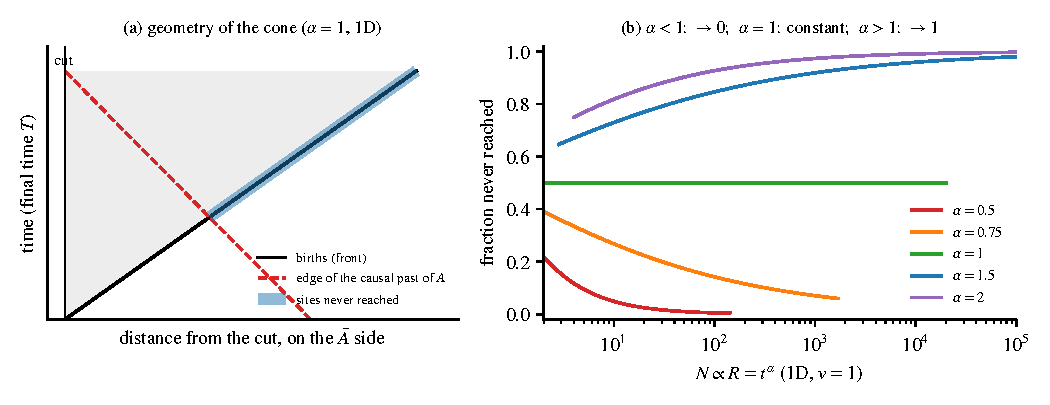
\includegraphics[width=\textwidth]{figures/fig_cone_geometry.pdf}
\caption{(a)~Geometry in one dimension for a linear front. A site is never reached (blue) if it is born beyond the edge of the causal past of the cut. (b)~Fraction of $\Abar$ out of reach as a function of size, for a front $R=t^\alpha$ and a causal speed $v=1$. It tends to $0$ if $\alpha<1$, stays constant (here $1/(1+v)$) if $\alpha=1$, and tends to $1$ if $\alpha>1$.}
\label{fig:cone}
\end{figure}

\begin{proposition}[front at constant speed, dimension $d$]\label{prop:front}
Consider a ball of radius $R(t)=st$ cut by a diametral hyperplane, and a cone of normal speed $v$. The fraction of $\Abar$ out of reach of the cone tends to
\begin{equation}\label{eq:fd}
f_d(\lambda)=\Big\langle 1-\Big(\frac{\lambda}{\lambda+u}\Big)^{d}\Big\rangle_{u},
\end{equation}
where $u$ is the direction cosine with respect to the normal, averaged over the hemisphere. One has $f_1=\frac{1}{1+\lambda}$, $f_3=1-\frac{\lambda(2\lambda+1)}{2(\lambda+1)^2}$ and $f_2=\frac1\pi\int_{-\pi/2}^{\pi/2}\big[1-\big(\frac{\lambda}{\lambda+\cos\theta}\big)^2\big]\dd\theta$. For every finite $\lambda$, $0<f_d(\lambda)<1$, and $f_d(\lambda)\sim d\langle u\rangle/\lambda$ as $\lambda\to\infty$.
\end{proposition}
\begin{proof}
A site at distance $r$ from the centre, with direction cosine $u>0$, is born at $t_x=r/s$. It is out of reach if and only if $ru>v(T-r/s)=\lambda(R-r)$, that is $r>\lambda R/(\lambda+u)$ (Coq lemmas \texttt{front\_not\_reached} and \texttt{front\_threshold}). In direction $u$, the fraction of volume beyond this radius is $1-(\lambda/(\lambda+u))^d$.
\end{proof}

In one dimension, with a birth at the edge every $k$ layers ($s=1/k$, $v=1$), $f_1=1/(1+k)$ and hence $G\ge\frac{N}{2}\frac{\log q}{1+k}-O(1)$. This is the absence of a threshold: the deficit stays extensive for every finite $k$.

\begin{remark}[Eden--Richardson model]\label{rem:eden}
In this model \cite{Eden1961,Richardson1973}, every empty site adjacent to the cluster is born at a constant rate $r>0$. The shape theorem \cite{Richardson1973,CoxDurrett1981} states that the cluster grows linearly with a convex limit shape. The birth times therefore satisfy $t_x=\mu(x)(1+o(1))$ for a norm $\mu$ invariant under the symmetries of the lattice, including the reflection through the cut, and a non-zero fraction of sites is out of reach, the analogue of \eqref{eq:fd} for the norm $\mu$. The shape theorem is used as a black box.
\end{remark}

\begin{proposition}[constant global rate]\label{prop:rate}
If sites are born at rate $\gamma$ per unit time inside a growing ball, so that $N=\gamma t$ and $R\propto t^{1/d}$, the number of sites of $\Abar$ out of reach is
\begin{equation}\label{eq:rate}
\#\{x\in\Abar:\ \mathrm d_\perp(x,A)>v(T-t_x)\}\simeq\frac{\gamma\,\omega_{d-1}}{d\,\omega_d\,v}\,R\;\propto\;N^{1/d},
\end{equation}
where $\omega_k$ is the volume of the unit ball in dimension $k$ (for $d=2$: $\gamma R/(\pi v)$). This number is extensive for $d=1$ and sub-extensive for $d\ge2$.
\end{proposition}
\begin{proof}
One has $\dot R=\gamma/(d\,\omega_dR^{d-1})$. A site at depth $\delta$ below the edge, at distance $\rho=Ru$ from the cut, was born a time $\delta/\dot R$ ago; it is out of reach if $\delta<\rho\dot R/v$. Integrate over the hemisphere of the edge, with $\int_{u>0}u\,\dd\Omega=\omega_{d-1}$.
\end{proof}

\begin{estimate}[homogeneous 1D expansion, continuum approximation]\label{est:homog}
Sites are inserted at uniformly random positions following a law $N(t)$. Assume that the comoving coordinate $u\in[0,1]$ of a site stays fixed (in reality it fluctuates as in a P\'olya urn). The cut is at $u=\frac12$ and the cone has speed $v$ in sites per unit time. A site born when the system had $N_b$ sites is out of reach if $u-\frac12>\Delta(N_b)=\int_{t_b}^Tv\,\dd t/N(t)$, and the fraction of $\Abar$ out of reach is $f=\frac{1}{N_T}\int\dd N_b\,(1-2\Delta)_+$. With $\tau=cN_0/v$:
\begin{itemize}[leftmargin=*,itemsep=1pt]
\item if $N=N_0(1+t/\tau)^{p}$ with $p<1$, then $\Delta\to\infty$ and $f\to0$;
\item if $p=1$, then $\Delta=c\ln(N_T/N_b)$ and $f=1-2c\,(1-e^{-1/(2c)})\in(0,1)$ (Coq lemmas \texttt{fraction\_p1\_pos} and \texttt{fraction\_p1\_lt1});
\item if $p>1$, then $\Delta\to0$ and $f\to1$; for exponential growth, about $v\tau\,[\ln(N_T/2v\tau)+O(1)]$ sites of $\Abar$ are reached.
\end{itemize}
\end{estimate}

The cases $p>1$ and exponential admit a simpler rigorous bound. Insertion preserves the order of the sites, so the sites of $A$ (the final left half) always form a prefix of the chain, and a single link separates $A$ from $\Abar$. A two-qudit gate across the cut increases $S(A)$ by at most $2\log q$. Hence $S(A)\le2\log q$ times the number of layers, that is $S(A)=O(N^{1/p})$ for $p>1$ and $S(A)\le2\tau\ln(N/N_0)\log q$ for exponential growth. The latter case is a random MERA run in the direction of growth: the $O(\log N)$ bound is Vidal's causal-cone bound \cite{Vidal2007,Vidal2008}, and the MERA has the causal structure of a discrete de Sitter space \cite{Beny2013,BaoDS2017}.

\begin{proposition}[sub-volume scaling laws]\label{prop:scaling}
Consider a circuit with $v$ layers per unit time and a region $A$ bounded by a planar cut of section $|\partial A(t)|\propto L(t)^{d-1}$. For a linear size $L\propto t^\alpha$ with $\alpha>1$,
\begin{equation}\label{eq:scaling}
S(A)\le C\,N^{\,1-\frac{\alpha-1}{\alpha d}} .
\end{equation}
For exponential growth ($L\propto e^{Ht}$), $S(A)\le C\,(v/H)\,L^{d-1}$ if $d\ge2$ (\emph{area law}) and $S(A)\le C\,(v/H)\ln L$ if $d=1$.
\end{proposition}
\begin{proof}
Every gate across the cut increases $S(A)$ by at most $2\log q$, and a layer contains at most $|\partial A(t)|$ such gates. Hence $S(A)\le2\log q\,v\int_0^T|\partial A(t)|\,\dd t\propto T^{\alpha(d-1)+1}$, while $N\propto T^{\alpha d}$. For a Hamiltonian, the entangling-rate bound of \cite{VanAcoleyen2013,Marien2016} gives the same result.
\end{proof}

Proposition~\ref{prop:scaling} follows directly from known area-times-time bounds and does not use the cone. For $\alpha\le1$ the same bound only gives $O(N)$, with no useful coefficient. It is in the marginal case $\alpha=1$ that the cone (Proposition~\ref{prop:front}) supplies the decisive information: a coefficient strictly below the maximum.

\begin{theoremL}\label{thm:C}
Consider isotropic front growth on $\mathbb Z^d$: a ball of radius $R(t)\propto t^\alpha$ cut by a diametral hyperplane, with growth symmetric under the reflection through this hyperplane (births in mirror pairs).
\begin{enumerate}[label=(\alph*),leftmargin=*]
\item If $\alpha\ge1$, then $G\ge c\,N-o(N)$ with $c>0$ for \emph{every} circuit of finite causal speed $v$ and, by Theorem~B, for every Lieb--Robinson dynamics on a fixed graph. One has $c=\frac12f_d(v/s)\log q$ for $\alpha=1$ and $c=\frac12\log q$ for $\alpha>1$.
\item If $\alpha<1$, there is a circuit of nearest-neighbour two-qudit gates, with $k$ layers per unit time ($k$ finite), such that $G=O(N\,T^{\alpha-1}/k)=o(N)$ at every time $T$.
\end{enumerate}
\end{theoremL}

\begin{proof}[Proof of (a); (b) is proven in Appendix~\ref{app:C}]
For $\alpha=1$, combine Corollary~\ref{cor:geo} and Proposition~\ref{prop:front}. For $\alpha>1$, Proposition~\ref{prop:scaling} gives $S=o(N)$. By symmetry, $|A|=|\Abar|$.
\end{proof}

The construction of (b) is a ``rainbow'' circuit \cite{Vitagliano2010}: in every row normal to the cut, newborn mirror pairs are brought side by side by an odd--even transposition sort, entangled into Bell pairs, and sent back; every Bell pair then straddles the cut. Only the sites born during the last cycle are unpaired, and a cycle lasts $O(R/k)$, a vanishing fraction of the age $T$ when $\alpha<1$.

\begin{remark}[extension normal to the cut]\label{rem:slab}
The criterion is about the extension \emph{normal} to the cut, not about linear size in general. Take a slab of fixed thickness $W$ that grows linearly parallel to the cut: $L\propto t$, but every site is within $W/2$ of the cut, and construction~(b), with rows of length at most $W$, gives $G=O(NW/(kT))=o(N)$.
\end{remark}

\begin{remark}[what a ``local growth rule'' means]\label{rem:local}
\begin{itemize}[leftmargin=*,itemsep=1pt]
\item \emph{Eden--Richardson}: $\alpha=1$, and the deficit is extensive for every local dynamics, in every dimension (Remark~\ref{rem:eden}).
\item \emph{Constant global rate}: $\alpha=1/d$, and the deficit is not guaranteed for $d\ge2$ (Theorem~C(b), Proposition~\ref{prop:rate}). Such a rate requires global coordination, or a single active site as in spiral growth.
\item \emph{Decelerated homogeneous expansion} ($N\propto t^p$, $p<1$, $d=1$): Estimate~\ref{est:homog} indicates that the cone catches up with everything; Theorem~A only guarantees an $O(1)$ deficit.
\end{itemize}
\end{remark}

%======================================================================
\section{Optimality in one dimension}\label{sec:A1}
%======================================================================

Consider edge growth with one birth every $k$ layers, up to $N=2m$, and $A=\{0,\dots,m-1\}$. The circuit has $L_f=k(2m-N_0)$ layers. Let $\delta_0=(m-L_f)\bmod 2$ and
\begin{equation}\label{eq:A1}
\mathcal{E}_k(m)=\Bigl\lfloor\frac{k(m+1)-\delta_0}{k+1}\Bigr\rfloor,\qquad D^\ast=2\mathcal{E}_k(m)-1+\delta_0 .
\end{equation}

\begin{proposition}[A1]\label{prop:A1}
(a) $|\Abar\cap\Inf(A)|=\mathcal{E}_k(m)$. Consequently $G(A)\ge(m-\mathcal{E}_k(m))\log q$ for every circuit.
(b) There is a brickwork Clifford circuit ($q=2$) for which $S(A)=\mathcal{E}_k(m)$ bits. The bound (a) is therefore optimal, and the minimal cut of the space-time network equals $\mathcal{E}_k(m)$.
\end{proposition}

\begin{proof}[Proof and status]
(a) The right edge of the causal past of $A$ starts at site $m-1$ and advances by one site per layer whenever the gate $(r,r+1)$ exists. Its $e$-th widening occurs at layer $L_f-\delta_0-e$ and requires site $m-1+e$ to be born, i.e. $k(m-1+e-N_0)\le L_f-\delta_0-e$. This condition is equivalent to $(k+1)e\le k(m+1)-\delta_0$, hence to $e\le\mathcal{E}_k(m)$.
(b) Construction: SWAP gates everywhere, except on the gate that straddles the cut, $(m-1,m)$, at depths $d=2j-1+\delta_0$ for $j=1,\dots,\mathcal{E}_k(m)$, where one applies $(H\otimes I)\cdot\mathrm{CNOT}$, which turns two fresh qudits into a Bell pair. The SWAPs carry the two halves along light rays. The left half is reflected by the fixed edge and stays in $A$, because $D^\ast\le 2m-1$; the right half is reflected by the moving edge and stays in $\Abar$. This gives $\mathcal{E}_k(m)$ Bell pairs across the cut.
\emph{Status.} The arithmetic inequalities used in (a) and (b) are proven in Coq without axioms (\texttt{ParityA1.v}): the condition for being alive, $e\le\mathcal{E}_k$, the bijection of depths, $\mathcal{E}_k\le m-1$, $D^\ast\le 2m-1$, $D^\ast\le km$, and monotonicity along the rays. The ray dynamics itself is not formalised. The construction is checked exhaustively by stabilizer simulation on $405$ cases ($k=1,\dots,8$; $N_0\in\{4,10,16\}$; $m\le60$; both values of $\delta_0$): measured cone $=$ formula $=S(A)$, with no failure. A maximum-flow computation on the space-time graph confirms that the minimal cut equals the cone in $24$ geometries ($k=1,\dots,6$, $N=60$ to $400$).
\end{proof}

For $k=1$, (a) gives $G\ge\lfloor m/2\rfloor\log q$, i.e.\ $G/(N\log q)\ge\frac14-O(1/m)$; in general $G/(N\log q)\ge\frac{1}{2(1+k)}-O(1/m)$. The lower end of the bracket of Corollary~\ref{cor:bracket} is thus attained, by a dynamics built for this purpose. Random circuits lie close to the upper end instead (Section~\ref{sec:num-edge}).

%======================================================================
\section{Typical dynamics: an exact single-wall model}\label{sec:walls}
%======================================================================

Theorems~A--C are worst-case statements. This section treats a typical dynamics: a brickwork chain in which every gate is drawn independently from a 2-design, with births at the right edge, and a region $A$ that is a prefix of the chain. The outcome is an exact description of the average purity of $A$ as a sum over the walks of a single domain wall that is absorbed by the line of births (Figure~\ref{fig:wall}).

\subsection{Assumptions and notation}

\paragraph{2-design.} Every gate follows a law $\nu$ on $U(q^2)$ whose second moment is that of the Haar measure:
\begin{equation}\label{eq:2design}
\E_{U\sim\nu}\bigl[U^{\otimes2}\otimes\bar U^{\otimes2}\bigr]=\E_{U\sim\mathrm{Haar}}\bigl[U^{\otimes2}\otimes\bar U^{\otimes2}\bigr].
\end{equation}
This holds for the Haar measure and for the uniform Clifford group when $q=2$ \cite{DLT2002,Dankert2009,Webb2016,Zhu2017}.

\paragraph{Geometry.} A birth at date $L$ adds a qudit $|0\rangle$ at the right edge just before layer $L$; the positions of existing qudits do not change. We take $A=\{0,\dots,m-1\}$ and $\Abar$ the rest, with $|\Abar|=N-m\ge m$, so that $G(A)=m\log q-S(A)$.

\paragraph{Annealed purity.} Let $Z_A=\E\,\mathrm{Tr}\,\rho_A^2$ and $\Srec(A)=-\log Z_A$. Since $S\ge S_2$ and $-\log$ is convex, Jensen's inequality gives
\begin{equation}\label{eq:jensen}
\E[S(A)]\ge\E[S_2(A)]\ge\Srec(A),\qquad\text{hence}\qquad \E[G(A)]\le m\log q+\log Z_A .
\end{equation}
All upper bounds on $\E[G]$ below are therefore bounds on the annealed quantity $m\log q+\log Z_A$; the gap between annealed and quenched averages, and between R\'enyi-2 and von Neumann entropies, is examined numerically in Section~\ref{sec:num-haar}.

\paragraph{Constants.} Let
\begin{equation}
K=\frac{q}{q^2+1},\quad a=\frac{q^2}{q^2+1},\quad b=\frac{1}{q^2+1},\quad v_B=a-b=\frac{q^2-1}{q^2+1},\quad E(v)=\log\frac1K-h\Bigl(\frac{1+v}2\Bigr),
\end{equation}
where $h(p)=-p\log p-(1-p)\log(1-p)$. Then $E(0)=-\log 2K=\log\frac{q^2+1}{2q}$, and the annealed entanglement velocity is $v_E^{(2)}=E(0)/\log q$, i.e.\ $0.3219$ for $q=2$. A direct computation gives
\begin{equation}\label{eq:EKL}
E(v)=|v|\log q+D_{\mathrm{KL}}\!\Bigl(\tfrac{1+|v|}{2}\,\Big\|\,a\Bigr)\ \ge\ \max\bigl(|v|\log q,\;E(0)\bigr),
\end{equation}
with equality $E(v)=|v|\log q$ if and only if $|v|=v_B$ (Coq proof of the equality: \texttt{butterfly\_tension}). $E(v)$ is the large-deviation cost per layer of a wall walk of velocity $v$ in the annealed model of Zhou and Nahum \cite{ZhouNahum2019}: its value at $v=0$ gives their annealed entanglement velocity $\tilde v_2=[\ln\frac{q^2+1}{q}-\ln2]/\ln q=v_E^{(2)}$, and the tangency $E(v_B)=v_B\log q$ is the general constraint on membrane tensions \cite{JHN2018,ZhouNahum2019,ZhouNahum2020}. It is not the quenched tension $\mathcal E_2(v)$, defined in the replica limit, nor the von Neumann tension; neither has a closed form at finite $q$.

\subsection{Input gauge}

For two copies, the permutations are $e$ (identity) and $s$ (swap). On a leg of dimension $q$ we write $\dket{\pi}$ for the associated vector, with $\langle\!\langle\pi|\pi'\rangle\!\rangle=q^{c(\pi^{-1}\pi')}$, i.e.\ $q^2$ if $\pi=\pi'$ and $q$ otherwise.

\begin{lemma}[Weingarten \cite{CollinsSniady2006}]\label{lem:wg}
Under \eqref{eq:2design}, $\E[U^{\otimes2}\otimes\bar U^{\otimes2}]=\sum_{\sigma,\tau\in\{e,s\}}\mathrm{Wg}(\sigma^{-1}\tau)\,\dket{\sigma\sigma}\dbra{\tau\tau}$, where $\sigma$ acts on the two output legs and $\tau$ on the two input legs, with $\mathrm{Wg}(e)=\frac{1}{q^4-1}$ and $\mathrm{Wg}(s)=-\frac{1}{q^2(q^4-1)}$.
\end{lemma}

\begin{lemma}[fresh leg]\label{lem:fresh}
For $\pi\in\{e,s\}$, $\langle\!\langle\pi|\,(|0\rangle\langle0|)^{\otimes2}\rangle\!\rangle=1$.
\end{lemma}
\begin{proof}
It is the trace of $\pi$ applied to two copies of a normalised pure state.
\end{proof}

For a gate $g$, follow each of its two output legs upwards to the first gate met, or to the upper boundary. Write $a_g^{\rm l},a_g^{\rm r}$ for the corresponding spins: either the input spin $\tau$ of that gate, or the boundary spin $\beta(x)$, which is $s$ if $x\in A$ and $e$ otherwise.

\begin{proposition}[input gauge]\label{prop:gauge}
\begin{equation}\label{eq:gauge}
Z_A=\sum_{\tau\in\{e,s\}^{\text{gates}}}\ \prod_g w\bigl(\tau_g;\,a_g^{\rm l},a_g^{\rm r}\bigr),\qquad
w(\tau;a,a')=\begin{cases}1 & a=a'=\tau,\\ K & a\ne a',\\ 0 & a=a'\ne\tau.\end{cases}
\end{equation}
\end{proposition}
\begin{proof}
Write $\mathrm{Tr}\,\rho_A^2=\langle\!\langle\beta|\,\rho^{\otimes2}\rangle\!\rangle$ and insert Lemma~\ref{lem:wg} for every gate (the three values of $w$ are checked in Coq: \texttt{w\_equal}, \texttt{w\_forbidden}, \texttt{w\_wall}). Independence of the gates turns the average into a product of moments. Input legs attached to a birth or to the initial state give~$1$ (Lemma~\ref{lem:fresh}), as do legs never touched. The output spin $\sigma_g$ appears only in $\mathrm{Wg}(\sigma_g^{-1}\tau_g)$ and in the two contractions of its output legs. Summing over $\sigma_g$, $w(\tau;a,a')=\sum_\sigma \mathrm{Wg}(\sigma^{-1}\tau)\,q^{c(\sigma^{-1}a)}q^{c(\sigma^{-1}a')}$, which equals $(q^4-1)/(q^4-1)=1$ if $a=a'=\tau$, $(q^2-q^2)/(q^4-1)=0$ if $a=a'\neq\tau$, and $q^3(1-q^{-2})/(q^4-1)=K$ if $a\ne a'$.
\end{proof}

The checks $Z_\emptyset=1$ (all boundary legs in $e$) and $Z_{\text{all}}=1$ (all in $s$) are immediate. The proposition depends neither on the dimension nor on the architecture: for every circuit of two-qudit gates drawn from a 2-design, on every graph and with arbitrary births, $Z_A$ is a sum of \emph{non-negative} weights. This fact is used in Section~\ref{sec:dimsup}.

\subsection{A single wall}

Process the events in reverse temporal order, keeping for each living leg the spin $a(x)$ of the first gate above it; initially $a=\beta$. Processing a gate on $(x,x+1)$ means choosing $\tau$ with weight $w(\tau;a(x),a(x+1))$ and setting $a(x)=a(x+1)=\tau$. Undoing a birth means removing the leg, with weight $1$. A \emph{wall} is a pair of neighbouring legs with different spins.

\begin{lemma}[no creation]\label{lem:creation}
No step of non-zero weight increases the number of walls, whether it is a gate or the removal of any leg (at the edge or in the bulk).
\end{lemma}
\begin{proof}
If $a(x)=a(x+1)$, the weight forces $\tau=a(x)$ and nothing changes. If $a(x)\ne a(x+1)$, the wall $(x,x+1)$ disappears and only one of the walls $(x-1,x)$ or $(x+1,x+2)$ can appear, since $\tau$ equals $a(x)$ or $a(x+1)$; the balance is $0$ or $-2$. Removing a bulk leg replaces two indicators by one, and $[a\ne c]\le[a\ne b]+[b\ne c]$. Formal proof: \texttt{walls\_nonincreasing} (\texttt{WallDescent.v}, no axiom).
\end{proof}

Zhou and Nahum established the weights $1$, $K$, $0$ and the absence of pair creation from the vacuum for a circuit of fixed size \cite{ZhouNahum2019}. Lemma~\ref{lem:creation} only adds the removal of legs.

\begin{proposition}[single-wall representation]\label{prop:single}
Let $A=\{0,\dots,m-1\}$, with births at the right edge. Label the wall by its position $p$: after the global symmetry $e\leftrightarrow s$, legs $[0,p)$ are in $e$ and legs $[p,n)$ in $s$. Start from $p=m$. Going down:
\begin{enumerate}[nosep]
\item a layer that contains the gate $(p-1,p)$ moves $p$ by $\pm1$, with weight $K$ in each direction; the other gates have weight~$1$;
\item removing leg $n-1$ sends $p$ to $\min(p,n-1)$;
\item the states $p=n$ and $p=0$ are absorbing: there is no wall left.
\end{enumerate}
$Z_A$ is the total weight of the walks once all events have been processed; all final states have weight $1$.
\end{proposition}

This follows from Proposition~\ref{prop:gauge} and Lemma~\ref{lem:creation}: a prefix has a single wall on the upper boundary, so every configuration of non-zero weight has at most one wall (\texttt{single\_wall} in Coq). A walk is \emph{in phase} when a gate straddles it, i.e.\ if $p-1\equiv L\pmod2$. A walk in phase stays in phase, because $p$ and the parity of the layer change together, and births at the right edge shift no position. Only the first layer can therefore be out of phase, and all living walks share the same phase.

\begin{figure}[t]
\centering
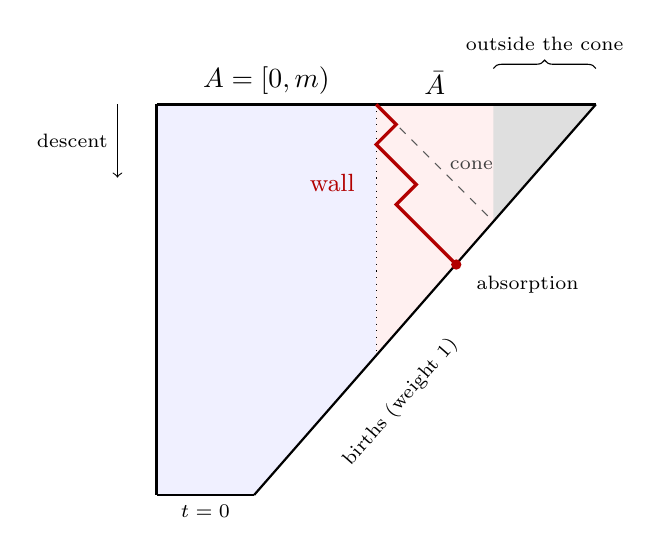
\begin{tikzpicture}[scale=0.62]
\fill[blue!6] (0,0) -- (2,0) -- (4.5,2.857) -- (4.5,8) -- (0,8) -- cycle;
\fill[red!6] (4.5,8) -- (9,8) -- (4.5,2.857) -- cycle;
\fill[gray!25] (6.9,5.6) -- (9,8) -- (6.9,8) -- cycle;
\draw[thick] (0,0) -- (0,8);
\draw[thick] (2,0) -- (9,8);
\draw[thick] (0,8) -- (9,8);
\draw[thick] (0,0) -- (2,0);
\draw[dotted] (4.5,8) -- (4.5,2.857);
\node[above] at (2.25,8) {$A=[0,m)$};
\node[above] at (5.7,8) {$\Abar$};
\draw[dashed,gray!70!black] (4.5,8) -- (6.9,5.6);
\node[gray!50!black,font=\scriptsize] at (6.45,6.75) {cone};
\draw[decorate,decoration={brace,amplitude=3pt,raise=13pt}] (6.9,8) -- (9,8) node[midway,above=16pt,font=\scriptsize] {outside the cone};
\draw[very thick,red!70!black] (4.5,8) -- (4.91,7.59) -- (4.5,7.18) -- (4.91,6.77) -- (5.32,6.36) -- (4.91,5.95) -- (5.32,5.54) -- (5.73,5.13) -- (6.14,4.72);
\fill[red!70!black] (6.14,4.72) circle (3pt);
\node[red!70!black,font=\small] at (3.6,6.4) {wall};
\node[font=\scriptsize,rotate=48.8] at (5.0,1.9) {births (weight $1$)};
\node[font=\scriptsize] at (7.6,4.3) {absorption};
\draw[->] (-0.8,8) -- (-0.8,6.5); \node[left,font=\scriptsize] at (-0.8,7.25) {descent};
\node[below,font=\scriptsize] at (1,0) {$t=0$};
\end{tikzpicture}
\caption{Edge growth in one dimension. Theorem~A bounds $G$ from below by the number of qudits of $\Abar$ born after the cone has passed (grey area): their world lines do not meet the causal past of $A$. For gates drawn from a 2-design, the average purity is a sum over the walks of a single wall (Proposition~\ref{prop:single}). The wall starts at the cut, makes $\pm1$ steps of weight $K$, and stops on the line of births, on the left edge, or at $t=0$.}
\label{fig:wall}
\end{figure}

\subsection{Exponential martingale}

\begin{lemma}[weight identity]\label{lem:weights}
For $j$ steps to the right and $l$ steps to the left, $K^{j+l}=q^{-(j-l)}\,a^j b^l$ (Coq: \texttt{weight\_identity}).
\end{lemma}

Let $\mathbb{P}_a$ be the law of the walk that moves right with probability $a$ and left with probability $b$ under each gate. Its velocity is $v_B$: it is the walk of the front of a spreading operator \cite{NVH2018,vK2018}. Let $X$ be the net displacement, counted only over the steps made under a gate, up to absorption or up to $t=0$.

\begin{corollary}[probabilistic representation]\label{cor:proba}
Exactly, $Z_A=\E_a\bigl[q^{-X}\bigr]=\E_b\bigl[q^{\,X}\bigr]$.
\end{corollary}
\begin{proof}
Each walk $\omega$ has weight $K^{j+l}=\mathbb{P}_a(\omega)\,q^{-X(\omega)}$ (Lemma~\ref{lem:weights}). The second form follows by exchanging $a$ and $b$.
\end{proof}

\begin{lemma}[bundle]\label{lem:bundle}
(a) $\binom{j+l}{j}K^{j+l}\le q^{-|j-l|}$ (Coq: \texttt{path\_bundle}, via the binomial identity $(a+b)^{j+l}=1$).
(b) The total weight of all paths of $t$ steps is $(2K)^t=e^{-tE(0)}\le1$ (Coq proof of $2K\le1$: \texttt{twoK\_le\_1}).
(c) $\binom{t}{j}K^t\le e^{-tE((2j-t)/t)}$, from the elementary bound $\binom tj\le e^{t\,h(j/t)}$ and $(1+v)/2=j/t$.
\end{lemma}

\subsection{Theorem D: recent births count the deficit}

Let $B(t)$ be the number of births with date $L\ge T-t$, i.e.\ during the last $t$ layers, endpoints included.

\begin{theoremL}\label{thm:D}
Assume a brickwork circuit, independent gates drawn from a 2-design, births at the right edge at arbitrary dates, and $A=\{0,\dots,m-1\}$ with $N-m\ge m$. Let $t^\ast=\lceil m\log q/E(0)\rceil=\lceil m/v_E^{(2)}\rceil$. If $T\ge t^\ast$, then
\begin{equation}\label{eq:thD}
Z_A\le\Bigl(2+\frac{1}{2K}\Bigr)\,q^{-(m-B(t^\ast))},\qquad
\E[G(A)]\le\log q\cdot B(t^\ast)+\log\Bigl(2+\frac{q^2+1}{2q}\Bigr).
\end{equation}
For $q=2$ the constant is $\log_2 3.25=1.70$ bits.
\end{theoremL}

The proof (Appendix~\ref{app:D}) classifies the walks by their stopping time: walks absorbed on the right before $t^\ast$ have travelled at least $m-B(t^\ast)$ sites and are suppressed by Corollary~\ref{cor:proba}; walks absorbed on the left are suppressed by $q^{-m}$; walks still alive after $t^\ast$ layers are suppressed by $(2K)^{t^\ast-1}$ (Lemma~\ref{lem:bundle}(b)).

\begin{proposition}[lower bound, every circuit]\label{prop:lower}
With births at the right edge and for every $s$ such that $s+B(s)\le m$, $G(A)\ge\log q\cdot B(s)$ for \emph{every} circuit.
\end{proposition}
\begin{proof}
The right edge of the causal past of $A$ moves by at most one site per layer; at date $L$ it lies at most at $m-1+(T-L)$. The births of the last $s$ layers occupy positions $x\ge N-B(s)\ge 2m-B(s)$, since $N\ge 2m$. They are outside the cone as soon as $2m-B(s)>m-1+s$, and they belong to $\Abar$. Conclude with Theorem~A.
\end{proof}

Thus $\log q\cdot B(\approx m)\le G$ and $\E[G]\le\log q\cdot B(m/v_E^{(2)})+O(1)$. For a 2-design dynamics, the mean deficit is bracketed by the births of two recent windows. The first lasts the light-crossing time ($m$ layers), the second the entanglement-crossing time ($m/v_E^{(2)}$, i.e.\ $3.11\,m$ for $q=2$). Older births have been ``digested''; more recent ones cannot be. This is a quantitative analogue, for this model, of Frautschi's horizon argument.

\begin{corollary}[summation for $\alpha<1$]\label{cor:alpha}
Consider births at the right edge with $n(L)-N_0=\lfloor L^\alpha\rfloor$, $0<\alpha<1$, and a final time $T$ such that $N=2m$. There are constants $C,c>0$, depending on $q$ and $\alpha$, such that for $m$ large enough
\begin{equation}
c\,m^{2-1/\alpha}-\log q\le\E[G(A)]\le C\,m^{2-1/\alpha}+C\quad(\tfrac12<\alpha<1),\qquad
\E[G(A)]\le C\quad(\alpha\le\tfrac12).
\end{equation}
In particular $\E[G]/N\to0$, and the exponent $2-1/\alpha$ is exact.
\end{corollary}
\begin{proof}
One has $T\simeq(2m-N_0)^{1/\alpha}\gg m$, so $t^\ast\le T/2$ for large $m$. By concavity, $B(t)\le T^\alpha-(T-t)^\alpha+1\le\alpha t(T/2)^{\alpha-1}+1$ for $t\le T/2$; with $t=t^\ast=O(m)$, Theorem~D gives the upper bound. For the lower bound, $B(s)\ge\alpha sT^{\alpha-1}-1$; take $s=\lfloor m/2\rfloor$, which satisfies $s+B(s)\le m$ for large $m$, and apply Proposition~\ref{prop:lower}.
\end{proof}

For $\alpha\le\frac12$, $m\log q-\Srec\to\log 2$ (Figure~\ref{fig:alpha}). This is the annealed Page correction \cite{Page1993}: $Z_A\simeq 2q^{-m}$, with one term from absorption on the right and one from absorption on the left, each of order $q^{-m}$.

\subsection{Theorem E: exact annealed density at $\alpha=1$}

\begin{theoremL}\label{thm:E}
Consider one birth every $k$ layers, as in Section~\ref{sec:A1}, with $N=2m$. Let $\theta_k\in(0,\log q)$ be the unique positive root of
\begin{equation}\label{eq:theta}
2K\cosh\theta=e^{-\theta/k}.
\end{equation}
Then, for $m$ large enough, $\tfrac12 e^{-2\theta_k}\,e^{-\theta_k m}\le Z_A\le (e^{2\theta_k}+2)\,e^{-\theta_k m}$, that is $\Srec(A)=\theta_k\,m+O(1)$. Moreover:
(a) $\theta_k=\min_{0\le v\le1}E(v)/(v+1/k)$;
(b) $\theta_1=\frac12\log\frac{q^2-q+1}{q}$, i.e.\ $0.2925$ bit per qudit for $q=2$ (Coq: \texttt{theta1\_root});
(c) $\theta_k<\log q\cdot\frac{kv_B}{1+kv_B}<\log q\cdot\frac{k}{k+1}$, and $\theta_k\to\log q$ as $k\to\infty$.
\end{theoremL}

The proof (Appendix~\ref{app:E}) uses the exponential martingale $h(D)=e^{-\theta_kD}$, where $D$ is the number of living legs to the right of the wall: \eqref{eq:theta} is exactly the condition for $h$ to be invariant under one period (one birth and $k$ layers) of the descent. Part (a) says that $\theta_k$ is the minimal cost of a wall that ends on the line of births, the exact counterpart, with an inclined absorbing boundary, of the membrane picture of \cite{ZhouNahum2019,ZhouNahum2020}.

\begin{proposition}[closed form for $k=1$]\label{prop:k1}
For $k=1$, $Z_A=\bigl(\frac{K}{1-K}\bigr)^{j^\ast}(1+O(e^{-cm}))$, where $j^\ast=m/2$ if $m$ is even and $j^\ast=(m\pm1)/2$ if $m$ is odd, depending on the phase of the first layer.
\end{proposition}
\begin{proof}
At $k=1$, each step back consists of one layer and one removal: $D$ decreases by $2$ (right step) or stays the same (left step). Absorption on the right happens at the $j^\ast$-th right step, and the negative binomial series gives $\sum_l\binom{j^\ast-1+l}{l}K^{j^\ast+l}=(K/(1-K))^{j^\ast}$. The excluded terms and the left and surviving contributions are exponentially smaller.
\end{proof}

\begin{corollary}[bracket at $\alpha=1$]\label{cor:bracket}
For gates drawn from a 2-design,
\begin{equation}\label{eq:bracket}
\frac{m-\mathcal{E}_k(m)}{2m}\le\frac{\E[G]}{N\log q}\le\frac12\Bigl(1-\frac{\theta_k}{\log q}\Bigr)+O\Bigl(\frac1m\Bigr),\qquad N=2m .
\end{equation}
The left bound tends to $\frac1{2(1+k)}$, holds for every circuit, and is attained (Proposition~\ref{prop:A1}). The right bound follows from Theorem~E and \eqref{eq:jensen}. As $q\to\infty$, $\theta_k/\log q\to k/(k+1)$ and the bracket closes on the minimal cut.
\end{corollary}

\begin{table}[h]
\centering\footnotesize\setlength{\tabcolsep}{4.5pt}
\begin{tabular}{c|cccc|cccc}
\toprule
 & \multicolumn{4}{c|}{$\theta_k/\log q$} & \multicolumn{4}{c}{bracket of $\E[G]/(N\log q)$} \\
$q$ & $k=1$ & $2$ & $4$ & $8$ & $k=1$ & $2$ & $4$ & $8$\\
\midrule
2 & 0.2925 & 0.4843 & 0.6760 & 0.8168 & [0.250, 0.354] & [0.167, 0.258] & [0.100, 0.162] & [0.056, 0.092]\\
3 & 0.3856 & 0.5814 & 0.7480 & 0.8603 & [0.250, 0.307] & [0.167, 0.209] & [0.100, 0.126] & [0.056, 0.070]\\
10 & 0.4795 & 0.6558 & 0.7946 & 0.8863 & [0.250, 0.260] & [0.167, 0.172] & [0.100, 0.103] & [0.056, 0.057]\\
\bottomrule
\end{tabular}
\caption{Values of $\theta_k$ (Theorem~E) and the bracket \eqref{eq:bracket} as $m\to\infty$.}
\label{tab:theta}
\end{table}

\begin{remark}[finite-size corrections]\label{rem:finitesize}
Theorem~E bounds the correction $c(m)=-\ln Z_A-\theta_km$ by $-\ln(e^{2\theta_k}+2)\le c(m)\le2\theta_k+\ln2$. The exact recursion ($q=2$; $k=1,2,4,8$; $N_0\in\{2,4,10\}$; $8\le m\le4097$) says more.
\begin{itemize}[leftmargin=*,itemsep=1pt]
\item $c(m)$ converges exponentially fast: $|c(m)-c(\infty)|<10^{-6}$ at the latest from $m=48$ ($k=1$), $49$ ($k=2$), $65$ ($k=4$) and $129$ ($k=8$), for the three values of $N_0$ and both parities of $m$.
\item The limit depends on the parity of $m$ but not on $N_0$. In nats: $c(\infty)=0$ and $-\theta_1$ for $k=1$ ($m$ even, odd), in agreement with Proposition~\ref{prop:k1}; $0.138$ and $-0.029$ for $k=2$; $0.199$ and $0.082$ for $k=4$; $0.249$ and $0.178$ for $k=8$.
\item The subleading constant is thus \emph{not universal}: it depends on microscopic details (the phase of the pattern when the wall arrives), while remaining bounded and small. The relative error on the density, $|{-\ln Z_A}/(\theta_km)-1|$, falls below $1\,\%$ from $m=33$ for $k\ge2$ and from $m=128$ for $k=1$ (because of odd $m$).
\end{itemize}
\end{remark}

\begin{remark}[membrane estimate]\label{rem:membrane}
A non-rigorous two-path estimate from the theory of entanglement membranes \cite{JHN2018,ZhouNahum2020} gives $dG/dN\gtrsim\frac12\max(1-kv_E,\,1/(1+kv_B))$: it compares the horizontal membrane (cost $v_E$ per layer) with the membrane that follows the front of an operator down to the line of births. The algebra of this estimate is checked in Coq (\texttt{ConeLemmas.v}); its premises, entropy bounded by the cost of each cut, are not. For a 2-design and the annealed tension, Theorem~E replaces the two extreme paths by the optimal one, $\min_vE(v)/(v+1/k)$. The same formula with an unknown quenched tension, convex and tangent at $v_B$, would give the unproven bracket $kv_E/(1+kv_E)\le\E[S]/m\le\min(kv_E,\,v_Bk/(1+v_Bk))$, in bits.
\end{remark}

\begin{remark}[structured dynamics]\label{rem:dualunit}
Theorems~D and~E assume a 2-design. Exploratory runs, \emph{not pre-registered}, on dual-unitary Clifford circuits ($\mathrm{SWAP}\cdot\mathrm{CZ}$ dressed with single-qubit gates) show that the position inside the bracket depends on the dressing. With random single-qubit dressing, $G=G_{\rm LB}$ exactly in $48$ points out of $48$ (edge growth, $k=1,\dots,4$, $N\le800$), so the lower bound is attained by a natural dynamics. The deterministic dressings $\mathrm{SWAP}\cdot\mathrm{CZ}$ and $\mathrm{SWAP}\cdot\mathrm{CZ}\cdot(H\otimes I)$ leave instead an extensive extra deficit; in the first case, qudits born in $|0\rangle$ are invariant under $\mathrm{CZ}$. Dual unitarity and maximal entangling power are therefore not enough: what matters is how the dynamics acts on the birth states.
\end{remark}

%======================================================================
\section{Higher dimensions: an obstruction and a conjecture}\label{sec:dimsup}
%======================================================================

In dimension $d\ge2$, Theorems~A and~C give the lower bound for every dynamics, but there is no analogue of Theorems~D and~E. The obstruction is precise.

\begin{proposition}[no monotonicity in dimension~2]\label{prop:obstruction}
On the square lattice, with two-qudit gates on the bonds, the input gauge keeps non-negative weights $1$, $K$, $0$, but neither the length of the wall (number of bonds between legs of different spins) nor the number of domains is monotone along the descent.
\end{proposition}
\begin{proof}
Take a gate on the horizontal bond $(x,y)$, with $a(x)=s$, $a(y)=e$, and the three other neighbours of $y$ in $e$. The choice $\tau=s$ has weight $K>0$ and puts $y$ in $s$: the number of wall bonds incident to $y$ goes from $1$ to $3$. If instead $a(x)=e$, $a(y)=s$, and $y$ joins two parts of an $s$ domain (its vertical neighbours in $s$, its opposite horizontal neighbour in $e$), the choice $\tau=e$, of weight $K$, cuts this domain in two. In one dimension both situations are impossible, because a site has only two neighbours (Lemma~\ref{lem:creation}).
\end{proof}

A wall therefore becomes a membrane that can grow and branch, and the problem no longer reduces to a walk with finitely many states. On a strip of width $w$ the annealed purity is still an exact transfer-matrix problem, but of dimension exponential in $w$.

\begin{conjecture}[membrane]\label{conj:membrane}
For an isotropic front at $\alpha=1$ in dimension~2, $-\log Z_A$ is, to leading order, the minimal cost $\int_\Sigma E_2(\hat n)\,\dd\sigma$ of a space-time surface $\Sigma$ anchored on $\partial A$ at time $T$ and free (weight $1$) on the surface of births, where $E_2$ is the annealed line tension of the 2D architecture. By scale invariance at $\alpha=1$, this predicts $-\log Z_A=N\,\Phi(\lambda)+o(N)$, where $\Phi$ depends only on $\lambda=v/s$.
\end{conjecture}

Theorem~E is the exact one-dimensional analogue of this conjecture. Three diagnostics are available and have not been carried out here. (i)~The spin model in the input gauge has no sign problem (Proposition~\ref{prop:gauge}), so Monte Carlo sampling of the configurations $\tau$ gives $Z_A$ in 2D far beyond the sizes accessible to state vectors. (ii)~The conjecture can be tested by the collapse of $-\log Z_A/N$ as a function of $\lambda$ alone, for several sizes. (iii)~Comparing with the quenched Clifford values of Table~\ref{tab:2d} would give the annealed--quenched gap in 2D.

%======================================================================
\section{Numerical tests}\label{sec:num}
%======================================================================

\subsection{Methods}\label{sec:num-methods}

\paragraph{Simulation.} States are stabilizer states, stored in a transposed, pre-allocated tableau whose generators are packed in 64-bit words \cite{AaronsonGottesman2004}. The entropy of a region is computed exactly as a rank over $\mathbb F_2$ \cite{Fattal2004}; for a stabilizer state the entanglement spectrum is flat, $S=S_2=S_\infty$. The strict cone $\Inf(A)$ is computed exactly by the backward sweep, with every gate recorded. Haar circuits ($q=2$, $N\le22$) are simulated as state vectors, and $S$ and $S_2$ are obtained from the Schmidt decomposition.

\paragraph{Gates.} The two-qubit Clifford group modulo Paulis is $\mathrm{Sp}(4,\mathbb F_2)$, of order $720$. Signs do not affect any entropy, so drawing the symplectic part uniformly reproduces the law of entropies under the uniform Clifford group, which is a 2-design \cite{DLT2002,Webb2016,Zhu2017}. We enumerated the $720$ matrices and checked closure of the group. The uniform Clifford group is even a 3-design \cite{Webb2016,Zhu2017}: the annealed averages of Theorems~D and~E are \emph{exactly} those of Haar; what can differ are quenched averages and the von Neumann entropy (Section~\ref{sec:num-haar}). One pitfall is worth reporting. The ensemble obtained by composing three layers of uniform elements of $\mathrm{SL}(2,\mathbb F_2)$ separated by two opposite CNOTs (``rand2'') reaches only $684$ of the $720$ elements, with multiplicities from $64$ to $144$ over the $6^6$ combinations: it is not a 2-design, and the purity test below rejects it. All values reported in this paper use uniform gates.

\paragraph{Statistics.} Averages are over independent circuits whose seeds are fixed in the scripts (Appendix~\ref{app:repro}). The standard error, given in parentheses on the last digits or after $\pm$, is the sample standard deviation (with Bessel's correction) divided by $\sqrt n$; the number $n$ of seeds is given in each caption. Slopes $dG/dN$ are fitted by least squares on each seed and then averaged; their standard error is that of the slopes between seeds. The exponents of Table~\ref{tab:2d} are log-log slopes between two sizes, computed on the means; their standard error is estimated by a bootstrap over seeds ($10^4$ resamplings). The lower (cone) and upper (annealed recursion) bounds at finite size are exact, so when a mean is compared with one of them the quoted uncertainty is purely statistical. Systematic uncertainties are finite-size effects: we do not extrapolate in $N$ except where the exact finite-size bound is available.

\paragraph{Pre-registration.} Every campaign was preceded by written, time-stamped predictions with success criteria (folder \texttt{preregistration/} of the repository). Predictions that failed are reported where they occur: the velocity threshold (Section~\ref{sec:num-edge}), two quantitative values for $N\propto t$ and the fast exponential front (Sections~\ref{sec:num-1d} and~\ref{sec:num-2d}), the agreement criterion between Haar and Clifford (Section~\ref{sec:num-haar}), the parity criterion at four seeds (Section~\ref{sec:num-1d}), one criterion for correlated births (Section~\ref{sec:num-correlated}) and one criterion of the free-field test (Section~\ref{sec:energy}). The repository's \texttt{preregistration/README.md} lists every prediction with its outcome.

\subsection{Checks of the 2-design and of the wall model}\label{sec:num-checks}

\emph{Single-wall recursion against the full model.} The recursion of Proposition~\ref{prop:single} was compared with an exact computation of the full spin model in the output gauge, which sums over the $3^n$ states with no assumption on walls. Over $18$ geometries ($q=2,3$; $N_0=2,\dots,5$; $n\le12$; $k=1,\dots,4$) and all cuts, the maximal relative deviation is $3.4\times10^{-15}$.

\emph{Uniform Clifford against the exact value.} For each of $9$ geometries, $2\times10^5$ circuits were drawn. The mean purity $\E[2^{-S(A)}]$ agrees with the exact $Z_A$ within $|z|\le2.3$. With rand2, the deviation is $z=+75$ to $+211$, the purity being $8$ to $54\,\%$ too high. The same check for Haar gates is reported in Table~\ref{tab:haar}.

\emph{Velocities.} The measured butterfly velocity (front of a Pauli operator, $200$ seeds) is $v_B=0.6004(42)$, against exactly $0.6$ for a 2-design \cite{NVH2018}. The quenched entanglement velocity, measured on a fixed chain of $512$ qubits with $8$ seeds, is $v_E=0.323(5)$ to $0.328(3)$ bit per layer depending on the fit window, just above the annealed value $v_E^{(2)}=0.3219$, which bounds it from below for every 2-design (Jensen's inequality, since $S=S_2$ for stabilizer states).

\emph{Theorem A.} No violation appears in $5632$ exact checks: $2400$ random Clifford circuits on random graphs with births, $2700$ Haar circuits with insertion, and $532$ checkpoints of the 1D and 2D campaigns of Sections~\ref{sec:num-1d} and~\ref{sec:num-2d}. The $261\,450$ circuits of Table~\ref{tab:haar} ($21\,450$ Haar, $240\,000$ Clifford) also satisfy it.

\subsection{Edge growth: no threshold, and the bracket}\label{sec:num-edge}

\begin{table}[h]
\centering\small\setlength{\tabcolsep}{4pt}
\begin{tabular}{rcccccc}
\toprule
$k$ & lower bound & uniform Clifford & upper bound & $\frac{\text{upper}-\E[G]}{\text{upper}}$ & Theorem E & membrane estimate\\
 & (cone, finite $m$) & $\E[G]/N$ & (recursion, finite $m$) & ($\%$) & $m\to\infty$ & $\frac12\max(1-kv_E,\frac{1}{1+kv_B})$\\
\midrule
1  & 0.2500 & 0.3516 (10) & 0.3538 & $+0.60\,(27)$ & 0.354 & 0.338\\
2  & 0.1665 & 0.2566 (5) & 0.2578 & $+0.46\,(18)$ & 0.258 & 0.227\\
4  & 0.0996 & 0.1616 (6) & 0.1618 & $+0.13\,(36)$ & 0.162 & 0.147\\
8  & 0.0552 & 0.0902 (2) & 0.0914 & $+1.38\,(18)$ & 0.092 & 0.086\\
16 & 0.0293 & 0.0487 (5) & 0.0484 & $-0.53\,(96)$ & 0.049 & 0.047\\
32 & 0.0146 & 0.0244 (0)$^\ast$ & 0.0248 & $+1.47$ & 0.025 & 0.025\\
\bottomrule
\end{tabular}
\caption{Edge growth, in bits per degree of freedom. Uniform Clifford: $N=2048$ and $6$ seeds for $k\le8$; $N=1024$ and $6$ seeds for $k=16$ and $32$. The lower and upper bounds are computed exactly at the same size; the column ``Theorem E'' gives the limit of the upper bound as $m\to\infty$. The membrane estimate, which is not a bound, uses $v_E=0.325$ and $v_B=0.6$. $^\ast$All six seeds give the same entropy ($487$ bits); the standard error is below $10^{-4}$.}
\label{tab:edge}
\end{table}

\begin{figure}[t]
\centering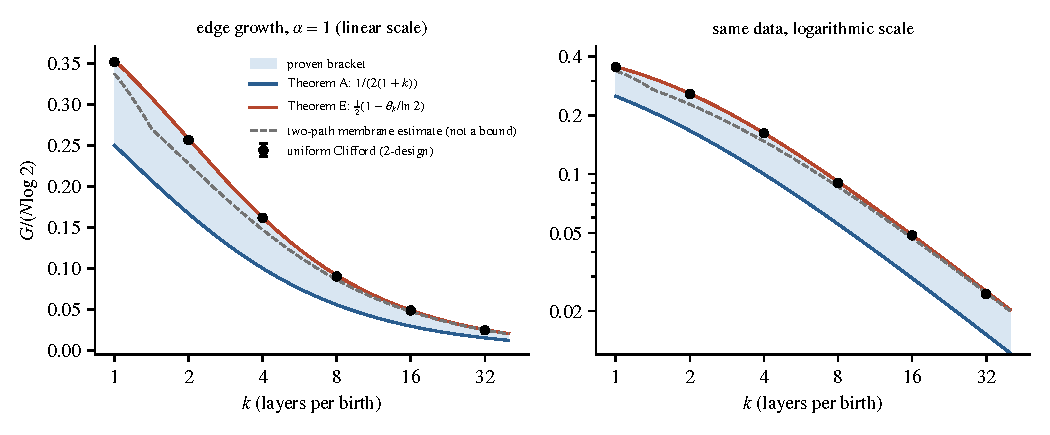
\includegraphics[width=\textwidth]{figures/fig_edge.pdf}
\caption{Edge growth ($\alpha=1$). The blue band is the proven bracket (Corollary~\ref{cor:bracket}). Black points: uniform Clifford circuits. Dashed: two-path membrane estimate. The deficit stays extensive for every $k$: the threshold prediction registered at the start, $k\,v_E\gtrsim\frac12$, is refuted.}
\label{fig:edge}
\end{figure}

Three observations stand out (Table~\ref{tab:edge}, Figure~\ref{fig:edge}).
(i)~There is no threshold: $G/N$ decreases like $1/k$ without ever vanishing, including when $kv_E$ is well above $\frac12$. The threshold prediction registered at the start is refuted.
(ii)~All values respect the proven bracket. Compared with the upper bound evaluated at the same size, they lie $0.13$ to $1.5\,\%$ below it; at $k=16$ the value exceeds the bound by $0.5\,\%$, i.e.\ $0.6$ standard error, which is compatible with Jensen's inequality. Equivalently, the quenched entropy density $\E[S]/m$ exceeds the exact annealed density by $0.0042(19)$, $0.0024(9)$, $0.0004(12)$ and $0.0025(3)$ bit per qudit for $k=1,2,4,8$ ($m=1024$); for $k=16$ and $32$ the difference is below $0.001$ bit.
(iii)~The two-path membrane estimate, which is not a bound, stays $3$ to $11\,\%$ below the data for $k\le16$ and exceeds them by $1.4\,\%$ at $k=32$. Theorem~E replaces it by a proven bound.
Stabilizer states have a flat entanglement spectrum ($S=S_2$); the next subsection compares with Haar gates at small sizes.

\subsection{Haar against Clifford at equal size}\label{sec:num-haar}

The uniform Clifford group gives exactly the annealed averages of Haar, but not necessarily the quenched ones, and its states have a flat entanglement spectrum. To separate these two effects, we simulated Haar circuits as state vectors in the exact geometry of Theorems~D and~E (edge growth, $N_0=2$, $A=[0,m)$, $N=2m$), and Clifford circuits in the same geometries (Table~\ref{tab:haar}). The predictions were written before the code.

\begin{table}[h]
\centering\footnotesize\setlength{\tabcolsep}{3.2pt}
\resizebox{\textwidth}{!}{%
\begin{tabular}{rrccccccccc}
\toprule
$N$ & $k$ & lower bound & Haar, $m-\E[S]$ & Clifford, $m-\E[S]$ & Haar, $m-\E[S_2]$ & upper bound & position $\varrho$ & $\E[S-S_2]$ (Haar) & annealed $z$\\
\midrule
12 & 1 & 3 & 3.904\,(3) & 4.101\,(5) & 4.251\,(4) & 4.274 & 0.71 / 0.86 / 0.98 & 0.347 & $-0.7$ / $+1.2$ \\
12 & 2 & 2 & 2.692\,(2) & 2.875\,(5) & 3.050\,(3) & 3.062 & 0.65 / 0.82 / 0.99 & 0.357 & $-0.3$ / $0.0$ \\
12 & 4 & 1 & 1.725\,(2) & 1.888\,(5) & 2.064\,(2) & 2.071 & 0.68 / 0.83 / 0.99 & 0.339 & $-1.8$ / $-1.1$ \\
16 & 1 & 4 & 5.223\,(5) & 5.454\,(5) & 5.644\,(6) & 5.673 & 0.73 / 0.87 / 0.98 & 0.422 & $-1.1$ / $-1.4$ \\
16 & 2 & 2 & 3.528\,(4) & 3.774\,(6) & 3.987\,(4) & 4.003 & 0.76 / 0.89 / 0.99 & 0.459 & $-0.5$ / $+0.2$ \\
16 & 4 & 1 & 2.200\,(3) & 2.398\,(5) & 2.567\,(3) & 2.576 & 0.76 / 0.89 / 0.99 & 0.366 & $-1.5$ / $+0.6$ \\
20 & 1 & 5 & 6.573\,(7) & 6.838\,(6) & 7.061\,(8) & 7.080 & 0.76 / 0.88 / 0.99 & 0.487 & $+0.2$ / $+0.8$ \\
20 & 2 & 3 & 4.508\,(6) & 4.760\,(6) & 4.992\,(6) & 5.006 & 0.75 / 0.88 / 0.99 & 0.484 & $-0.2$ / $+0.1$ \\
20 & 4 & 2 & 2.745\,(3) & 2.928\,(5) & 3.121\,(4) & 3.124 & 0.66 / 0.83 / 1.00 & 0.376 & $+0.6$ / $+0.2$ \\
22 & 1 & 6 & 7.556\,(18) & 7.834\,(6) & 8.046\,(21) & 8.078 & 0.75 / 0.88 / 0.98 & 0.489 & $-0.4$ / $+0.3$ \\
22 & 2 & 4 & 5.219\,(15) & 5.487\,(6) & 5.720\,(17) & 5.741 & 0.70 / 0.85 / 0.99 & 0.501 & $-0.4$ / $-1.0$ \\
22 & 4 & 2 & 3.140\,(11) & 3.352\,(5) & 3.558\,(12) & 3.561 & 0.73 / 0.87 / 1.00 & 0.418 & $+0.4$ / $-0.8$ \\
\bottomrule
\end{tabular}}
\caption{Mean deficit (bits) in the geometry of Theorems~D and~E, $q=2$. Haar: $4000$, $2000$, $1000$ and $150$ circuits for $N=12$, $16$, $20$ and $22$; Clifford: $2\times10^4$ circuits per geometry. Lower (cone) and upper ($m+\log_2Z_A$) bounds are exact. Position $\varrho=(\E[G]-\text{lower})/(\text{upper}-\text{lower})$ for Haar--von Neumann, Clifford and Haar--R\'enyi-2. $z$: deviation of $\E[2^{-S_2}]$ from the exact $Z_A$, in standard errors, for Haar and Clifford.}
\label{tab:haar}
\end{table}

\begin{itemize}[leftmargin=*,itemsep=1pt]
\item \emph{Checks.} The mean purity agrees with the exact $Z_A$ in every geometry ($|z|\le1.8$). No circuit violates Theorem~A.
\item \emph{Ordering.} In every geometry, $\E[G]$ for Haar--von Neumann $<$ $\E[G]$ for Clifford $<$ $m-\E[S_2]$ for Haar $\le$ upper bound. The positions inside the bracket are $0.65$--$0.76$ (Haar, von Neumann), $0.82$--$0.89$ (Clifford) and $0.98$--$1.00$ (Haar, R\'enyi-2).
\item \emph{Haar R\'enyi-2.} The quenched mean $\E[S_2]$ exceeds the annealed value by only $0.003$ to $0.032$ bit: for Haar, Jensen's inequality $\E[S_2]\ge\Srec$ is nearly saturated, and Theorem~E predicts the quenched R\'enyi-2 entropy to this accuracy.
\item \emph{Haar von Neumann.} The difference $D(m)=\E[S]-\E[S_2]$ is $0.34$ to $0.50$ bit. It grows with $m$, but more and more slowly for $k=1$ ($0.35$, $0.42$, $0.49$, $0.49$ bit at $N=12$, $16$, $20$, $22$); for $k=4$ it keeps growing ($0.38$ then $0.42$ bit at $N=20$ and $22$). Weighted fits of $D(m)$ by $a+bm$, $a+b\ln m$ and $a-b/m$ (\texttt{haar\_vs\_clifford\_analysis.py}) are all poor, with $\chi^2\ge21$ for $2$ degrees of freedom for every $k$; the last point ($m=11$) is the only odd $m$, and parity effects of the kind seen in Remark~\ref{rem:finitesize} are a plausible cause. The data therefore do not discriminate between a bounded $D(m)$ and one that grows linearly with a small slope, which is what the theory of random circuits suggests (see below).
\item \emph{Clifford} is intermediate: its entropy, equal to its R\'enyi-2 entropy, exceeds the quenched Haar R\'enyi-2 entropy by $0.15$ to $0.23$ bit, a difference that varies little between $N=20$ and $22$.
\item \emph{Pre-registration.} Four criteria are confirmed (annealed check; $\E[S]>\E[S_2]$ and growth with $m$; ordering Haar--von Neumann $<$ Clifford; higher position for Clifford). The criterion $|\E[S_2]_{\rm Haar}-\E[S]_{\rm Clifford}|\le0.2$ bit \emph{fails} from $N=16$ on, with at most $0.23$ bit.
\end{itemize}
At these sizes the width of the bracket (about two bits) is comparable to the differences between ensembles, so the position $\varrho$ depends on the ensemble and on the entropy chosen. Densities are another matter, and the two entropies should be treated separately. For R\'enyi-2, the quenched--annealed difference is expected to be small: in random circuits of fixed size it comes from interactions between replicas and is parametrically small at large $q$ \cite{ZhouNahum2019}, in agreement with the $0.003$ to $0.032$ bit observed here and with the Clifford data at large size. For the von Neumann entropy there is no such expectation. At finite $q$ the entanglement velocity, and more generally the line tension, depends on the R\'enyi index, and the dependence disappears only as $q\to\infty$ \cite{ZhouNahum2019}. Transposed to Theorem~E, whose density $\theta_k$ is the minimal cost of a wall ending on the line of births, this suggests (heuristically) that at $q=2$ the von Neumann density differs from the annealed R\'enyi-2 density by an amount of order one per site, i.e.\ that $D(m)$ grows linearly in $m$ with a small slope; the data (linear slopes $0.03$ bit per site for $k=1,2$ and $0.01$ for $k=4$, with poor fits) neither confirm nor exclude this. What is proven is unaffected: since $S\ge S_2$, the bracket of Corollary~\ref{cor:bracket} holds for the von Neumann entropy, and only the position inside it is open. What is established numerically is that the annealed bound predicts the quenched Haar R\'enyi-2 entropy to a few hundredths of a bit, and R\'enyi-2 is the quantity estimated by randomised-measurement protocols \cite{Brydges2019}.

\subsection{Births in pairs}\label{sec:num-pairs}

\begin{table}[h]
\centering\small
\begin{tabular}{rccccc}
\toprule
$k$ & R (pure qudit) & P1 (local pair) & P2 (non-local pair) & R/P2 & R/P2, minimal cut\\
\midrule
0  & 0.5000 & 0.5000 & 0.2486 (72) & 2.01 (6) & 2\\
1  & 0.3515 (11) & 0.3521 (6) & 0.1575 (53) & 2.23 (8) & 2.05\\
2  & 0.2559 (8) & 0.2565 (5) & 0.0874 (61) & 2.93 (20) & 2.76\\
4  & 0.1600 (4) & 0.1614 (7) & 0.0459 (27) & 3.49 (20) & 3.09\\
8  & 0.0912 (3) & 0.0911 (2) & 0.0268 (20) & 3.40 (25) & 3.09\\
16 & 0.0483 (2) & 0.0484 (4) & 0.0134 (12) & 3.61 (33) & 4.12\\
32 & 0.0252 (3) & 0.0249 (1) & 0.0051 (8) & 4.90 (74) & ---\\
\bottomrule
\end{tabular}
\caption{Slope $dG/dN$ (bit per degree of freedom), fitted on $N\in[200,800]$, uniform Clifford, $8$ seeds, edge growth. Scrambling is $k$ layers per added degree of freedom in all three variants. Last column: the same ratio for the exact minimal cut of the space-time network ($n\le160$, $3$ seeds; the value at $k=0$ is exact).}
\label{tab:pairs}
\end{table}

Suppose each distinction creates a Bell pair; there are two cases (Table~\ref{tab:pairs}).
\emph{Local pair (P1).} The slope is indistinguishable from the reference for every $k$, within $1.7$ standard errors. The birth condition does not require each degree of freedom to be born pure; it requires it to be born without \emph{long-range} correlation with the pre-existing world (Remark~\ref{rem:pairs} and Section~\ref{sec:num-correlated}).
\emph{Non-local pair (P2):} one member is born at the edge, the other inserted at a uniformly random position. Without scrambling ($k=0$), the added deficit is $\frac14$ per degree of freedom instead of $\frac12$, because one pair in two straddles the cut. With scrambling, the weakening R/P2 goes from $2.2$ to $3.6$ for $k=1,\dots,16$, and is $4.9\pm0.7$ at $k=32$; this last value lies outside the announced interval $[2,4.5]$ while remaining compatible with it within one standard error. The slope stays positive: the arrow is weakened, not erased. An exact minimal cut of the space-time network, in which each Bell pair is a link that the cut must cross (\texttt{mincut\_pairs.py}), gives ratios of $2.05$ to $4.12$ for $k=1,\dots,16$, within about $15\,\%$ of the measured ones, but at smaller sizes ($n\le160$). The geometry of the shortcuts thus accounts for the order of magnitude of the effect; the residual differences, of either sign, are not explained here.

\subsection{Births correlated with the past}\label{sec:num-correlated}

\begin{table}[h]
\centering\small\setlength{\tabcolsep}{5pt}
\begin{tabular}{lcccccc}
\toprule
 & $f=0$ & $0.01$ & $0.03$ & $0.1$ & $0.3$ & $1$\\
\midrule
$k=1$, non-local & 0.3518 (5) & 0.3485 (14) & 0.3435 (14) & 0.3332 (45) & 0.2828 (44) & 0.1415 (40)\\
$k=1$, local & & & & 0.3514 (7) & & 0.3521 (8)\\
$k=4$, non-local & 0.1597 (6) & 0.1602 (7) & 0.1575 (11) & 0.1521 (15) & 0.1264 (16) & 0.0604 (28)\\
$k=4$, local & & & & 0.1609 (4) & & 0.1612 (8)\\
\bottomrule
\end{tabular}
\caption{Slope $dG/dN$ (bit per degree of freedom) on $N\in[200,800]$, edge growth, uniform Clifford, $8$ seeds. With probability $f$, the newborn undergoes at birth a uniform Clifford gate with an existing site: its immediate neighbour (local) or an existing site drawn uniformly (non-local). The mean mutual information between the newborn and the past, just after a correlated birth, is $1.6$ bit (non-local) and $0.9$ to $1.6$ bit (local).}
\label{tab:correlated}
\end{table}

Table~\ref{tab:correlated} quantifies Proposition~\ref{prop:births}(c) and Remark~\ref{rem:pairs}.
\begin{itemize}[leftmargin=*,itemsep=1pt]
\item \emph{Local correlation:} even with $f=1$ and a mutual information of order one bit per birth, the slope does not change ($|\text{difference}|\le1.7$ standard errors). The amount of correlation with the past is not the relevant variable.
\item \emph{Non-local correlation:} the slope decreases with $f$. For $f\le0.1$, each correlated birth costs on average $0.2$ to $0.3$ bit of deficit for $k=1$ and about $0.08$ bit for $k=4$, less than the instantaneous bound $\frac12I\approx0.8$ bit of Proposition~\ref{prop:births}(c), which takes into account neither the position of the partner nor the subsequent scrambling. At $f=1$ the slope is divided by $2.5$ ($k=1$) and $2.6$ ($k=4$), but stays positive by more than $20$ standard errors: the arrow is weakened, not erased.
\item \emph{Pre-registration:} the announced criteria are met, except the relative reduction at $f=0.1$ for $k=4$, which is $4.8(10)\,\%$ for an announced interval $[5\,\%,75\,\%]$; the miss is smaller than one standard error.
\end{itemize}

\subsection{Annealed and quenched; the regime $\alpha<1$}\label{sec:num-alpha}

\begin{figure}[t]
\centering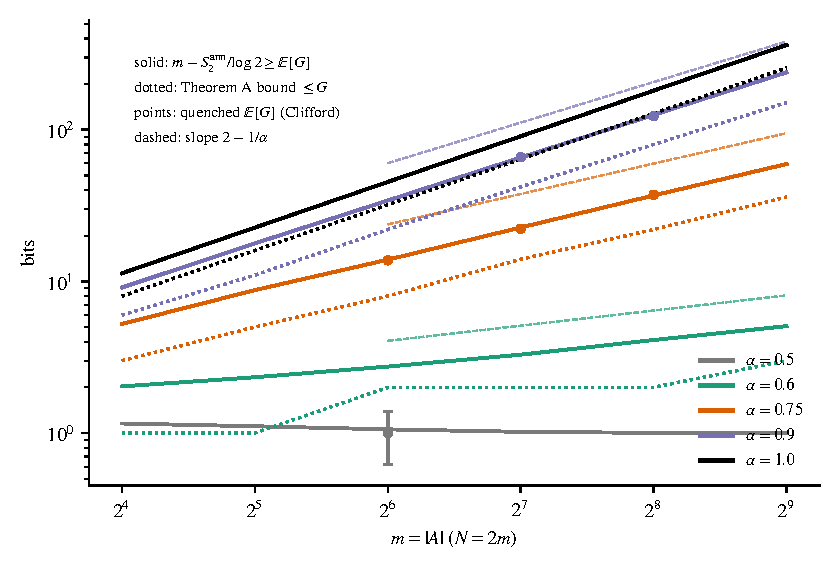
\includegraphics[width=0.72\textwidth]{figures/fig_alpha.pdf}
\caption{Growth $n-N_0=\lfloor L^\alpha\rfloor$. Solid: $m-\Srec/\log2$, an exact upper bound on $\E[G]$. Dotted: the lower bound of Theorem~A, valid for every circuit. Points: quenched $\E[G]$ for uniform Clifford circuits ($8$ seeds). Dashed: slope $2-1/\alpha$ of Corollary~\ref{cor:alpha}.}
\label{fig:alpha}
\end{figure}

\emph{Exact annealed density.} The exact recursion, computed in the log domain, gives $-\log_2 Z_A/m=0.29248$, $0.48428$, $0.67606$ and $0.81682$ for $k=1,2,4,8$ at $m=16\,384$. The agreement with $\theta_k/\ln2$ is within $0$ to $2\times10^{-5}$, and the correction $-\log Z_A-\theta_km$ converges to a constant, as Theorem~E predicts. At $k=1$, the ratio $Z_A\,(3/2)^{m/2}$ equals $1.000000$ for even $m$ from $m=40$ on, and $(3/2)^{\pm1/2}$ for odd $m$, depending on the phase (Proposition~\ref{prop:k1}).

\emph{Regime $\alpha<1$.} For $\alpha\in\{0.4,0.5,0.6,0.75,0.9,1\}$ and $m=16$ to $512$, with up to $10^6$ layers, the chain ``bound~A $\le m-\Srec/\log2\le B(t^\ast)+1.70$'' holds in all $34$ cases, with a minimal margin of $0.70$ bit (Figure~\ref{fig:alpha}). The log-log slopes over the three largest $m$ are $0.42$, $0.72$ and $0.94$ for $\alpha=0.6$, $0.75$ and $0.9$, against the proven asymptotic exponents $0.33$, $0.67$ and $0.89$; the difference is expected at these sizes. For $\alpha\le\frac12$, $m-\Srec/\log 2\to1$ bit. The quenched Clifford values ($8$ seeds) are $13.75(25)$, $22.25(25)$ and $37.25(37)$ bits for $\alpha=0.75$ and $m=64$, $128$, $256$, to be compared with the annealed bounds $13.90$, $22.67$ and $36.86$; the last point exceeds its bound by $1.1$ standard errors, which is compatible.

\subsection{Insertion in one dimension and parity locking}\label{sec:num-1d}

\begin{table}[h]
\centering\small
\begin{tabular}{lcccccc}
\toprule
growth & $G/N$ ($400$) & $G/N$ ($1600$) & $G_{\rm LB}/N$ ($1600$) & prediction ($v=1$) & with $v_{\rm eff}$ & $S$ ($1600$) \\
\midrule
edge, $k=1$ & $0.347$ & $0.3502\,(12)$ & $0.2500$ & $0.250$ & --- & $240\,(2)$ \\
edge, $k=4$ & $0.161$ & $0.1595\,(9)$ & $0.1000$ & $0.100$ & --- & $545\,(2)$ \\
$N\propto t^{1/2}$ & $0.015$ & $0.0033\,(4)$ & $0.0020\,(4)$ & $0.001$ & $0.001$ & $795\,(1)$ \\
$N\propto t$ & $0.411$ & $0.4155\,(15)$ & $0.2711\,(36)$ & $\mathbf{0.184}$ & $0.261$ & $135\,(2)$ \\
$N\propto t$, pairs & $0.341$ & $0.3381\,(11)$ & $0.1889\,(13)$ & $0.184$ & $0.184$ & $259\,(2)$ \\
$N\propto t^2$ & $0.487$ & $0.4919\,(4)$ & $0.4777\,(12)$ & $0.455$ & $0.477$ & $13\,(1)$ \\
$N\propto e^{t/\tau}$ & $0.488$ & $0.4962\,(10)$ & $0.4883\,(10)$ & $0.477$ & $0.489$ & $6\,(2)$ \\
\bottomrule
\end{tabular}
\caption{Uniform Clifford, 1D, $N_0=16$, $c=\frac12$, four seeds. Prediction: Estimate~\ref{est:homog} with $v=1$; column $v_{\rm eff}$: the same formula with the effective velocity of the strict cone, measured on $44$ seeds. The value in bold is a quantitative prediction that failed. The row ``pairs'' is the control added afterwards (insertions in adjacent pairs).}
\label{tab:1d}
\end{table}

\begin{itemize}[leftmargin=*,itemsep=1pt]
\item \emph{Decelerated} ($N\propto t^{1/2}$): $G\approx5$ bits at $N=1600$, and the bound is $3$ sites. The deficit stays bounded, as in Corollary~\ref{cor:alpha}, which treats edge growth; the case of insertion is not covered by a proof.
\item \emph{Linear} ($N\propto t$): the deficit is extensive and stable, as predicted. But the bound is $G_{\rm LB}/N=0.271$ instead of the predicted $0.184$, and $G/N=0.416$ lies outside the pre-registered interval $[0.18,0.40]$. \emph{Both quantitative predictions fail.}
\item \emph{Mechanism, formulated afterwards and then tested: parity locking.} Going back in time from $A$, the set reached is a prefix $[0,b]$ of the chain. After each layer its edge is aligned with the next layer of the brickwork pattern. Each insertion at a position $\le b$ shifts $b$ by one unit and flips this alignment. \emph{The edge therefore advances by one site if and only if the number of insertions to its left since the previous layer is even.} This rule holds in $100\,\%$ of the $7378$ unsaturated layers. It is purely combinatorial: the strict cone depends only on the structure of the circuit, so $v_{\rm eff}$ does not depend on the law of the gates. It does depend on the architecture (a two-layer pattern) and on the statistics of insertions.
\item \emph{Closed form.} For $r$ independent uniform insertions between two layers, the probability of an even number of insertions to the left of the edge is $\frac12[1+(1-2\pi)^r]$, where $\pi=(b+1)/n$ is the fraction of the chain to the left of the edge. Averaging this expression along the realisations gives $v_{\rm eff}=0.583$, $0.500$, $0.501$ and $0.969$ for $N\propto t$, $t^2$, $e^{t/\tau}$ and $t^{1/2}$, against $0.583(3)$, $0.504(9)$ and $0.488(13)$ measured on $44$ seeds, and $0.969(6)$ on four seeds for $t^{1/2}$. The registered prediction, agreement within $0.02$ on the four initial seeds, fails for $t^2$ ($0.546(30)$ measured) and for exponential growth ($0.472(42)$): these two laws offer only $284$ and $144$ unsaturated layers. With $44$ seeds, added afterwards, the agreement is within one standard error. For edge growth and pair insertions, the number of insertions to the left of the edge is always even and $v_{\rm eff}=1$.
\item \emph{Control predicted in advance.} Insertions in adjacent pairs preserve parity. One then measures $v_{\rm eff}=1.000$ and $G_{\rm LB}/N=0.189$, against $0.184$ predicted, a deviation of $+3\,\%$ within the announced margin of $\pm5\,\%$.
\item \emph{Accelerated}: $G/N\to\frac12$ and $S$ stays small ($13$ and $6$ bits at $N=1600$), in agreement with the $O(N^{1/2})$ and $O(\log N)$ bounds of Section~\ref{sec:geo}.
\end{itemize}

\subsection{Two dimensions}\label{sec:num-2d}

\begin{table}[h]
\centering\small
\begin{tabular}{lcccccc}
\toprule
growth & $G/N$ ($400$) & $G/N$ ($1600$) & $G/N$ ($6400$) & $G_{\rm LB}/N$ ($6400$) & prediction & exponent of $G$ \\
\midrule
front $s=\frac14$ & $0.077\,(2)$ & $0.0741\,(8)$ & $0.0742\,(1)$ & $0.0691$ & $0.069$ & $1.001\,(7)$ \\
front $s=\frac12$ & $0.137\,(2)$ & $0.1387\,(13)$ & $0.1360\,(4)$ & $0.1244$ & $0.123$ & $0.986\,(6)$ \\
front $s=1$ & $0.239\,(2)$ & $0.2370\,(15)$ & $0.2241\,(7)$ & $0.1966$ & $0.199$ & $0.960\,(5)$ \\
Eden $r=\frac14$ & $0.160\,(10)$ & $0.132\,(10)$ & $0.134\,(4)$ & $0.116\,(3)$ & ($0.119$) & $1.01\,(5)$ \\
Eden $r=1$ & $0.316\,(10)$ & $0.313\,(8)$ & $0.317\,(9)$ & $0.271\,(8)$ & ($0.281$) & $1.01\,(1)$ \\
rate $\gamma=16$ & $0.0825$ & $0.0391\,(2)$ & $0.0187\,(1)$ & $0.0180$ & $0.018$ & $0.468\,(4)$ \\
rate $\gamma=4$ & $0.0225\,(10)$ & $0.0091\,(2)$ & $0.0046$ & $0.0043$ & $0.004$ & $0.512\,(14)$ \\
\bottomrule
\end{tabular}
\caption{Uniform Clifford, 2D. Four seeds; eight independent clusters per rate for Eden; standard errors in parentheses (omitted when below one unit of the last digit). The bound of Theorem~A is identical from one seed to the next for fronts and constant rate. The exponent of $G$ is the slope of $\ln G$ against $\ln N$ between $1600$ and $6400$, with a bootstrap standard error over seeds. The prediction, fixed in advance, is $f_2(2/s)/2$ for fronts and $\gamma R/(2\pi N)$ for the constant rate. For Eden, in parentheses, the same formula uses the front velocity measured afterwards.}
\label{tab:2d}
\end{table}

\begin{figure}[t]
\centering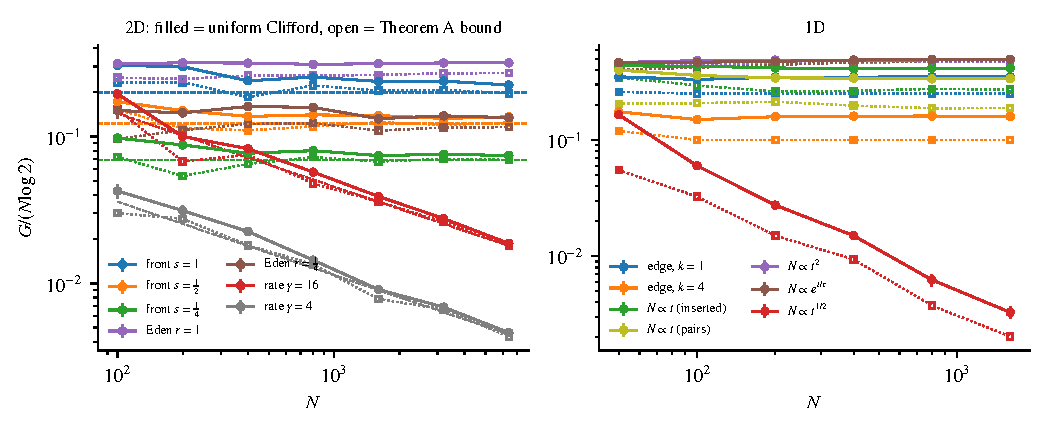
\includegraphics[width=\textwidth]{figures/fig_dichotomy.pdf}
\caption{Deficit per degree of freedom, uniform Clifford. Filled symbols: simulation. Open symbols: bound of Theorem~A computed exactly for each realisation. Dashed (2D): analytic predictions $f_2(2/s)/2$ and $\gamma R/(2\pi N)$. Left (2D): fronts and Eden keep a constant $G/N$, whereas the constant rate decreases like $N^{-1/2}$. Right (1D): decelerated insertion is the only class that tends to~$0$.}
\label{fig:dichotomy}
\end{figure}

\begin{itemize}[leftmargin=*,itemsep=1pt]
\item \emph{Fronts and Eden}: the deficit is extensive, and $G/N$ is stable to a few per cent between $N=1600$ and $6400$. At $N=6400$ the measured bound agrees with $f_2(\lambda)/2$ to better than $2\,\%$, with no fitted parameter. The random circuit nearly reaches the bound: $G/G_{\rm LB}$ is $1.07$ to $1.17$, so the strict cone captures $85$ to $93\,\%$ of the observed deficit.
\item \emph{Constant rate}: $G/N$ decreases by a factor $\approx2$ for each quadrupling of $N$. The exponent of $G$ is $0.468(4)$ and $0.512(14)$, inside the pre-registered interval $[0.3,0.75]$. A constant global rate does not produce an extensive arrow in dimension~2.
\item \emph{Scaling laws} (Figure~\ref{fig:scaling}): between $N=1600$ and $6400$ the local exponent of $S$ is $0.82$ and $0.85$ for the $t^2$ fronts (bounds $0.84$ and $0.87$). These values are sub-volume, but still above the asymptotic value $\frac34$. The exponent is $0.66$ for the slow exponential front (bound $0.72$). The fast exponential front ($H=1$ per round) \emph{fails} as a test: no gate crosses the cut between $N=1600$ and $6400$, because growth is faster than the gate cadence. The criterion used to choose this parameter omitted this condition.
\end{itemize}

\begin{figure}[t]
\centering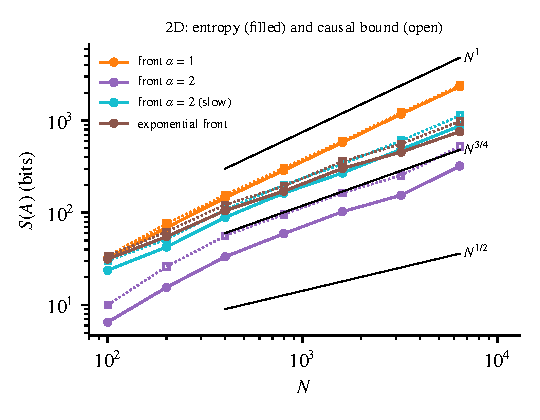
\includegraphics[width=0.5\textwidth]{figures/fig_scaling.pdf}
\caption{Entropy of one half (filled symbols) and causal bound (open symbols) in 2D, uniform Clifford. The linear front follows a volume law. The accelerated fronts ($R=at^2$) are clearly sub-volume, in their pre-asymptotic regime.}
\label{fig:scaling}
\end{figure}

%======================================================================
\section{The energy cost of the birth condition}\label{sec:energy}
%======================================================================

The qudit register has no Hamiltonian and no vacuum: being born uncorrelated costs nothing there. In a theory with a vacuum, the birth of an uncorrelated mode is a local quench, whose energy can be compared with the energy created by expansion. Foster and Jacobson concluded, for a massless field on a growing lattice, that local mode birth injects too much energy into the vacuum to be a viable model of cosmological mode creation \cite{FosterJacobson2004}. We quantified this cost for three birth rules, one of which is the analogue of the birth condition of this paper.

\paragraph{Model.} A free scalar field of mass $m$ on a periodic 1+1D lattice, with cutoff $\Lambda=1$ and a physical spacing $\ell(t)\in[1,2]$ that follows $a(t)\propto t^{1/2}$, $t^3$ or $e^{Ht}$. The Hamiltonian is $\sum_i[P_i^2/(2\ell)+(\phi_{i+1}-\phi_i)^2/(2\ell)+\ell m^2\phi_i^2/2]$. When $\ell$ reaches $2$, every cell is refined by the canonical Haar map $\phi_{2i,2i+1}=\phi_i\pm w_i/2$, $P_{2i,2i+1}=P_i/2\pm p_i$; the pairs $(w_i,p_i)$ are the newborn degrees of freedom. The computation is exact (Gaussian covariance matrices, $N\le2048$). Three rules are compared.
\begin{itemize}[leftmargin=*,itemsep=1pt]
\item \emph{R1, product}: every newborn is born in the ground state of its local oscillator, uncorrelated with the rest. This is the birth condition of this paper.
\item \emph{R2, vacuum-preserving}: the Gaussian isometry $S=\mathrm{diag}(M,M^{-T})$, with $M=X_1^{1/2}X_0^{-1/2}$, maps the coarse vacuum ($X_0=2\Gamma_\phi$ of the reference state) exactly to the fine vacuum ($X_1$).
\item \emph{R3, MERA}: R1 followed by $D$ layers of translation-invariant two-site Gaussian gates optimised to minimise the energy.
\end{itemize}

\begin{table}[h]
\centering\small\setlength{\tabcolsep}{4.5pt}
\resizebox{\textwidth}{!}{%
\begin{tabular}{lccccc}
\toprule
rule & $\varepsilon/\Lambda$ per newborn & quanta per newborn & dependence on $H$ & MI with existing cells & $G_E/|A|$ (de Sitter)\\
\midrule
R1, product & $0.066$--$0.084$ & $0.044$--$0.057$ & none & $0$ ($<10^{-15}$) & $0.26$--$0.30$\\
R3, MERA $D=2$ & $6.4\times10^{-4}$ & $5.4\times10^{-4}$ & none & $0.15$ nat, slow tail & $0.017$--$0.018$\\
R3, MERA $D=4$ & $5.6\times10^{-5}$ & --- & --- & --- & ---\\
R2, vacuum-preserving & $\le3.5\times10^{-6}$ & $0$ ($<3\times10^{-15}$) & $\propto H^{1.97}$ & $0.16$ nat & $(5$--$7)\times10^{-3}$\\
\bottomrule
\end{tabular}}
\caption{Free field on an expanding lattice, $m=0.05$, $H\in[0.0025,0.2]$. $\varepsilon$: excitation energy injected per newborn. MI: mutual information between a newborn and all existing cells other than its mother cell, just after birth ($N_c=512$). $G_E=S_{\rm th}(A;E)-S(A)$: gap between the entropy of one half and the thermal entropy at the same energy, in nats per site, for $H=0.05$ and $N=128$ to $1024$. For comparison, expansion alone creates about $0.6\,(H/\Lambda)^2$ instantaneous quanta per site and per doubling.}
\label{tab:energy}
\end{table}

\paragraph{Results} (Table~\ref{tab:energy}; the predictions were written before the code).
\begin{itemize}[leftmargin=*,itemsep=1pt]
\item \emph{R1} injects $\approx0.053$ quanta, i.e.\ $\approx0.08\,\Lambda$, per newborn, independently of $H$ and of the expansion law; from the exact vacuum, $\varepsilon=0.0696\,\Lambda$, independent of $N$. This is about $0.09\,(\Lambda/H)^2$ times the production by expansion: $1.5\times10^4$ times at $H=0.0025$, and the ratio diverges as $H/\Lambda\to0$. The quanta of R1 are at the cutoff scale and those of expansion are infrared, so the difference is even larger in energy.
\item \emph{R3} reduces the cost (from $6.96\times10^{-2}$ to $5.6\times10^{-5}\,\Lambda$ for $D=0$ to $4$) without making it depend on $H$: a finite depth is not enough. The pre-registered prediction that $\varepsilon$ would stay above $10^{-3}\Lambda$ for $D\le3$ \emph{failed}, as too pessimistic: the threshold is crossed at $D=2$.
\item \emph{R2} injects almost nothing ($\varepsilon\propto H^{1.97}$) and conserves the number of quanta exactly (Proposition~\ref{prop:quanta}). But it is \emph{correlated with the past}: $0.16$ nat of mutual information between a newborn and the existing cells other than its mother cell, and $0.080$ nat of total entanglement per newborn with the existing cells. From the exact vacuum these correlations decay like $e^{-2mr}$, and the matrix elements of $M$ decay exponentially, over about $15$ sites: R2 is a \emph{local} correlated birth in the sense of Proposition~\ref{prop:births}(c). The entropy of one half stays in an area law, close to that of the vacuum, and the gap $G_E$ only measures the excess adiabatic energy due to expansion, of standard origin.
\end{itemize}

\begin{proposition}[R2 conserves quanta]\label{prop:quanta}
For every coarse Gaussian state, rule R2 exactly conserves the number of instantaneous quanta $Q=\frac12\mathrm{Tr}(\Gamma_\phi X^{-1})+\frac12\mathrm{Tr}(\Gamma_P X)-\frac N2$, where $X=2\Gamma_\phi^{\rm vac}$.
\end{proposition}
\begin{proof}
Since $MX_0M^{T}=X_1$, $\mathrm{Tr}(M\Gamma_\phi M^TX_1^{-1})=\mathrm{Tr}(\Gamma_\phi X_0^{-1})$ and $\mathrm{Tr}(M^{-T}\Gamma_PM^{-1}X_1)=\mathrm{Tr}(\Gamma_PX_0)$. The newborns, in their local state, contribute $0$ to $Q$ before the map is applied. Numerical check on random excited states: deviation $\le4\times10^{-15}$.
\end{proof}
The non-zero energy injected by R2 therefore comes only from the redistribution of pre-existing quanta between frequencies, whose density is itself $\propto H^2$.

\paragraph{Translation to 3+1 dimensions, under an assumption.} Suppose that an R1 birth also costs $\varepsilon\Lambda$ in 3+1 dimensions, with $\varepsilon\approx0.08$; we have not computed this. With a fixed physical cutoff, births occur at a rate $3H\Lambda^3$ per unit volume and inject $3H\varepsilon\Lambda^4$ per unit volume and time. This radiation dilutes as $a^{-4}$, giving an equilibrium density $\rho^\ast=\frac34\varepsilon\Lambda^4$. The Friedmann equation requires $\rho^\ast\le3H^2M_{\rm Pl}^2$ ($M_{\rm Pl}$ the reduced Planck mass), that is
\begin{equation}\label{eq:cutoff}
\Lambda\lesssim(4/\varepsilon)^{1/4}(HM_{\rm Pl})^{1/2}\approx2.7\,(HM_{\rm Pl})^{1/2},
\end{equation}
about $5$~meV for the present Hubble rate ($H_0\approx1.4\times10^{-33}$~eV). Such a cutoff is excluded experimentally. The conclusion is insensitive to the assumed value of $\varepsilon$, which enters only as $\varepsilon^{-1/4}$: a cost a hundred times smaller raises the bound by a factor $3.2$, and a cutoff above $1$~TeV would require $\varepsilon\lesssim10^{-58}$, that is, an essentially vacuum-preserving birth. The conclusion agrees with that of Foster and Jacobson \cite{FosterJacobson2004}, and the R1/R2 dichotomy is that of the debate on trans-Planckian initial states: a state that respects adiabaticity leaves only corrections of order $(H/\Lambda)^2$ \cite{KKLS2002}, whereas a birth in the instantaneous vacuum at the cutoff, which is not adiabatic, costs energy \cite{Danielsson2002,MartinBrandenberger2001}.

\paragraph{Scope and limits.} The birth condition that produces the arrow of this paper is therefore excluded, in a theory with a vacuum, by its energy cost, and the admissible rule is locally correlated with the past and carries no deficit of its own. The test has limits: a free field does not scramble (the gap $G_E$ contains a floor specific to free fields, whose mode occupations are conserved); it is 1+1-dimensional; $H/\Lambda\ge2.5\times10^{-3}$ is far from cosmological values, and the extrapolation relies on the measured scaling laws; only one refinement map (Haar) was studied. How the cost decreases when the range of the birth correlations is truncated, between R1 (range zero) and R2 (range of order $1/m$), was not studied; the MERA results show that a finite depth lowers the cost by orders of magnitude without making it depend on $H$. The energy argument itself does not depend on the dynamics: interactions redistribute the injected energy, they do not remove it.

%======================================================================
\section{Discussion}\label{sec:discussion}
%======================================================================

\subsection{What is established, and how firmly}

The starting question was whether a register that creates uncorrelated degrees of freedom catches up with its maximal entropy when scrambling is fast. It receives an answer at three levels.
\begin{enumerate}[leftmargin=*,itemsep=2pt]
\item \emph{For every dynamics}, the deficit is bounded below by the number of degrees of freedom born outside the causal past of the region (Theorem~A). This is a statement about causality, independent of the scrambling rate.
\item \emph{For the geometry of growth}, what matters is the extension normal to the cut compared with causal propagation. At least linear growth guarantees an extensive deficit. Slower growth leaves the cone time to catch up with everything, and a well-chosen dynamics can then close the deficit (Theorem~C). The bound is optimal in one dimension (Proposition~A1).
\item \emph{For a typical dynamics} (2-design), the mean deficit is set, up to constants, by the births of two recent windows of durations $m$ and $m/v_E^{(2)}$ (Theorem~D). For linear growth, the annealed density is known exactly (Theorem~E). For Clifford circuits, the simulations place the quenched value within $1.5\,\%$ of this bound evaluated at the same size; for Haar circuits at $N\le22$, the quenched R\'enyi-2 entropy nearly saturates it and the von Neumann entropy lies about half a bit away, a gap that the theory of random circuits suggests is extensive with a small density (Section~\ref{sec:num-haar}).
\end{enumerate}
The Frautschi-type velocity criterion (relaxation against expansion), which served as the initial prediction and was refuted, is thus replaced by a \emph{horizon} criterion: the question is not whether scrambling is fast, but whether a finite fraction of the degrees of freedom is born outside the causal past of the cut. Table~\ref{tab:status} states, for each result, whether it is proven, what is checked in Coq, and what rests on cited results or on non-formalised arguments.

\begin{table}[h]
\centering\footnotesize\setlength{\tabcolsep}{3.5pt}
\begin{tabular}{p{3.6cm}p{2.4cm}p{4.3cm}p{4.7cm}}
\toprule
statement & status & checked in Coq & not formalised, or cited\\
\midrule
Theorem~A & proven & splitting of the circuit (\texttt{split\_*}) & quantum step: the four facts of Remark~\ref{rem:quantumfacts}\\
Corollary~\ref{cor:geo}, Props.~\ref{prop:front}, \ref{prop:rate}, \ref{prop:scaling} & proven & front thresholds (\texttt{front\_*}) & volume integrals\\
Estimate~\ref{est:homog} & heuristic & sign of the fraction ($p=1$) & continuum approximation (P\'olya urn neglected)\\
Theorem~B & proven & --- & Lieb--Robinson bound cited \cite{NSY2019}; Duhamel; Fannes--Audenaert\\
Theorem~C & proven & --- & (a) Eden: shape theorem cited; (b) odd--even sort cited\\
Proposition~A1 & proven & arithmetic (\texttt{ParityA1.v}) & ray dynamics (checked on $405$ cases)\\
Proposition~\ref{prop:births} & proven & --- & Araki--Lieb\\
Prop.~\ref{prop:gauge} (input gauge) & proven & weights $1,0,K$ (\texttt{w\_*}) & Weingarten values cited \cite{CollinsSniady2006}\\
Lemma~\ref{lem:creation}, Prop.~\ref{prop:single} & proven & \texttt{walls\_nonincreasing}, \texttt{single\_wall} & ---\\
Corollary~\ref{cor:proba}, Lemma~\ref{lem:bundle} & proven & \texttt{weight\_identity}, \texttt{path\_bundle}, \texttt{twoK\_le\_1} & (c): $\binom tj\le e^{t\,h(j/t)}$\\
Theorem~D, Corollary~\ref{cor:alpha} & proven & --- & summations, concavity\\
Theorem~E, Prop.~\ref{prop:k1} & proven & $\theta_1$, $E(v_B)=v_B\log q$ & finite martingale identity (induction), Legendre transform\\
Proposition~\ref{prop:obstruction} & proven & --- & ---\\
Prop.~\ref{prop:quanta} (free field) & proven & --- & ---\\
Conjecture~\ref{conj:membrane} (2D) & conjecture & --- & ---\\
Remarks~\ref{rem:membrane}, \ref{rem:finitesize} & heuristic; exact numerics & algebra of the estimate (\texttt{ConeLemmas.v}) & premises of the estimate\\
\bottomrule
\end{tabular}
\caption{Status of the statements. ``Proven'': complete proof in the text or the appendices, possibly from cited results. The numerical tests (Section~\ref{sec:num}) also test the proven statements.}
\label{tab:status}
\end{table}

\subsection{The birth condition}

The arrow obtained is not derived from nothing. It follows from the fact that no degree of freedom is born correlated at \emph{long range} with the existing register. The birth state itself matters little: any fixed pure state will do (Proposition~\ref{prop:births}(a)). Local correlations with the past do not change the density of the deficit, even when they reach one bit per birth (Remark~\ref{rem:pairs}, Tables~\ref{tab:pairs} and~\ref{tab:correlated}). Non-local correlations weaken it by a factor $2$ to $5$ without removing it.

Section~\ref{sec:energy} shows the price of this condition in a theory with a vacuum: an uncorrelated birth costs an energy of the order of the cutoff, and the birth compatible with the vacuum is locally correlated with the past and carries no deficit of its own. In its admissible version, the birth condition therefore coincides with the usual assumption that modes crossing the cutoff are born in their adiabatic vacuum \cite{BunchDavies1978,MartinBrandenberger2001}. It does not displace the past hypothesis: the origin of the low entropy remains in the initial state, and first of all in its gravitational degrees of freedom, which dominate the entropy budget \cite{Penrose1989,EganLineweaver2010}.

\subsection{Cosmological reading (a constrained analogy)}

\begin{itemize}[leftmargin=*,itemsep=1pt]
\item For $\alpha<1$ (decelerated expansion), the comoving horizon grows without bound and everything eventually comes into causal contact. A scrambling dynamics can then close the deficit at the rate at which regions enter the horizon. A 2-design dynamics does, with a residual deficit $\Theta(m^{2-1/\alpha})$ if $\alpha>\frac12$ and $O(1)$ otherwise (Corollary~\ref{cor:alpha}).
\item For $\alpha>1$ (accelerated expansion), an event horizon separates regions for good. An accelerated phase produces a maximal deficit, with an area-law entropy (Proposition~\ref{prop:scaling}).
\item The marginal case $\alpha=1$ (``coasting'' expansion) has no event horizon: the comoving horizon diverges logarithmically. The extensivity of the deficit is a measure effect, since a finite fraction of the sites was born recently, near the edge.
\end{itemize}
These readings describe the causal geometry of a register that grows by uncorrelated births. In a field theory such births are excluded by their energy cost (Section~\ref{sec:energy}), and the boundary $\alpha=1$ does not coincide exactly with the existence of an event horizon. We do not claim that this model describes the universe. The natural domain of the results is that of quantum processors into which fresh ancilla qubits enter during the computation.

\subsection{Prior work and positioning}\label{sec:prior}

\begin{itemize}[leftmargin=*,itemsep=2pt]
\item \emph{Light-cone and entangling-rate bounds.} The generation of correlations and entanglement is limited by the Lieb--Robinson cone \cite{BHV2006,EisertOsborne2006}, and the growth rate of entropy is bounded by the area of the cut \cite{Bravyi2007,VanAcoleyen2013,Marien2016}. Theorem~A is an elementary case of the first kind; Theorem~B follows \cite{BHV2006} with the bound of \cite{NSY2019}; Proposition~\ref{prop:scaling} follows from the second kind.
\item \emph{Random circuits.} Entanglement growth and its membranes \cite{NRVH2017,JHN2018,ZhouNahum2020,Sierant2023}, operator spreading \cite{NVH2018,vK2018}, and the domain-wall model for the purity with its free boundary \cite{ZhouNahum2019} are used as they are. The function $E(v)$ is the annealed cost of a wall walk of Zhou and Nahum, and Theorem~E is its exact version with an inclined absorbing boundary: $\theta_k=\min_vE(v)/(v+1/k)$ is the minimal cost of a wall that stops on the line of births. Our contribution is limited to treating births as this lateral absorbing boundary and to deriving from it the exact single-wall representation and Theorems~D and~E.
\item \emph{MERA and de Sitter.} The logarithmic (1D) or area-law bound of MERA follows from its causal cone \cite{Vidal2007,Vidal2008}, and MERA has the causal structure of a discrete de Sitter space \cite{Beny2013,BaoDS2017}. Our exponential case coincides with this setting.
\item \emph{Growing Hilbert spaces in cosmology}: \cite{Jacobson1999,Bao2017,CotlerStrominger2022,Cao2023}. These models create or bring in unentangled degrees of freedom without analysing the deficit as a function of scrambling or the role of locality.
\item \emph{Open systems.} Piroli, S\"underhauf and Qi study a system coupled to an environment by random circuits (Hayden--Preskill protocol) \cite{PSQ2020}. Circuits with resets, which inject fresh qudits by \emph{replacing} existing ones, show a phase transition \cite{Yokoyama2026}. Our births add degrees of freedom without removing any: that is the essential difference.
\item \emph{Random growth}: the Eden--Richardson model and the shape theorem \cite{Eden1961,Richardson1973,CoxDurrett1981}. \emph{Rainbow states}: volume-law entanglement from concentric singlets \cite{Vitagliano2010}.
\item \emph{Arrow of time and entanglement}: \cite{AlKhaliliChen2024}. \emph{Growing entropy ceiling}: \cite{Layzer1975,Frautschi1982}.
\item \emph{Energy cost of mode births}: growing lattice \cite{FosterJacobson2004}; trans-Planckian initial states \cite{MartinBrandenberger2001,Danielsson2002,KKLS2002}. Section~\ref{sec:energy} recovers and quantifies this constraint; it is not new.
\end{itemize}
What seems specific to this work comes down to five points: the analysis of the marginal case $\alpha=1$ in any dimension, with the resulting dichotomy; parity locking; exact optimality in one dimension; the single-wall representation in the presence of births, with Theorems~D and~E; and the distinction between the range and the amount of birth correlations. Everything follows from known tools: these are new applications, not a new theory. Targeted literature searches (October 2026) did not find these statements; absence of evidence is not evidence of absence, and review by a specialist remains necessary.

\subsection{Limitations}

\begin{itemize}[leftmargin=*,itemsep=1pt]
\item \emph{Non-2-design dynamics.} Theorems~D and~E assume a 2-design. For other dynamics, only the bracket by Theorem~A and the trivial bound remain, and the position inside it depends on the dynamics: a randomly dressed dual-unitary circuit attains the lower bound (Remark~\ref{rem:dualunit}).
\item \emph{Annealed, quenched, R\'enyi.} Theorems~D and~E bound $\E[G]$ through Jensen's inequality. For Clifford circuits, the measured quenched--annealed difference is at most $0.004$ bit per qudit. For Haar circuits, the difference between von Neumann and R\'enyi-2 entropies is about half a bit at $N\le22$ (Table~\ref{tab:haar}). Since line tensions depend on the R\'enyi index at finite $q$, this difference is probably extensive; we can neither compute its density nor bound it, and fits at these sizes do not decide. The bracket itself holds for the von Neumann entropy.
\item \emph{Region.} Theorems~D and~E only treat prefixes. For a union of $r$ intervals, Lemma~\ref{lem:creation} bounds the number of walls by $2r$, but annihilations complicate the summation.
\item \emph{Bulk births.} Lemma~\ref{lem:creation} still applies, but an insertion shifts the phase of the legs to its right. One must then replace $t^\ast-1$ by $t^\ast-1-B(t^\ast)$ in the proof of Theorem~D. The statement remains true if $B(t^\ast)=o(t^\ast)$, but this is not written out here. For decelerated insertion we only have the continuum estimate and the numerical data.
\item \emph{Higher dimensions.} The wall becomes a non-monotone membrane (Proposition~\ref{prop:obstruction}). The typical case in 2D remains a conjecture.
\item \emph{Worst case.} Theorem~C only treats isotropic fronts; its ``only if'' direction is established by construction; the Eden case rests on the shape theorem, used as a black box; Theorem~B assumes a fixed host graph.
\item \emph{Simulations.} Large sizes use $q=2$ and Clifford gates; Haar circuits are limited to $N\le22$. A single architecture is studied per dimension, and the effective causal velocity depends on it (parity locking).
\item \emph{Physics.} The model has no energy. In a theory with a vacuum, the birth condition that produces the arrow is excluded by its energy cost (Section~\ref{sec:energy}).
\end{itemize}

\subsection{Open problems}

\begin{enumerate}[leftmargin=*,itemsep=2pt]
\item \emph{Experimental test.} A quantum processor can add qubits mid-circuit by bringing in freshly prepared ancillas, and the mean purity $\E\,\mathrm{Tr}\,\rho_A^2$ can be measured with randomised measurements \cite{Brydges2019}. For gates drawn from a 2-design, Theorem~E gives its exact value with no adjustable parameter: $-\log_2\E\,\mathrm{Tr}\,\rho_A^2=\theta_k m/\ln2+c(m)/\ln 2$, with the constants of Remark~\ref{rem:finitesize}.
\item \emph{Robustness beyond 2-designs.} Characterise the position inside the bracket for approximate designs, for structured circuits (dual-unitary, matchgate, Floquet) and for Hamiltonian dynamics, beyond the examples of Remark~\ref{rem:dualunit}.
\item \emph{Typical case in 2D.} Sample the spin model in the input gauge, which has no sign problem, by Monte Carlo, and test the membrane conjecture (Section~\ref{sec:dimsup}).
\item \emph{Quenched and von Neumann entropies.} Compute the von Neumann analogue of $\theta_k$, i.e.\ the minimal cost of a von Neumann membrane ending on the line of births, by a replica method or in an expansion in $1/q$, and the quenched--annealed correction to the R\'enyi-2 density.
\item \emph{Correlated births.} Establish a bound that depends on the geometry of birth correlations, and not only on their maximal range.
\end{enumerate}

\subsection{Conclusion}

In a quantum register that grows by pure, uncorrelated births, the gap to maximal entropy does not close because scrambling is fast. It can close only if the causal past of the region catches up with the births; for a typical dynamics in one dimension, it then does close. The mean deficit counts the births of a recent window whose duration lies between one light crossing and one entanglement crossing. An extensive arrow exists as soon as the first window contains a finite fraction of the degrees of freedom; for a typical dynamics, it disappears as soon as the second contains a vanishing fraction. This result was obtained by replacing a velocity prediction, registered and then refuted, by a proven horizon criterion. It is robust to the birth state and to local correlations with the past. It does not, however, solve the cosmological problem of the arrow of time: in a theory with a vacuum, births without correlation with the past cost an energy of the order of the cutoff, and the birth compatible with the vacuum carries no deficit of its own.

\appendix
%======================================================================
\section{Proofs}\label{app:proofs}
%======================================================================

\subsection{Theorem B}\label{app:B}

\paragraph{The Lieb--Robinson bound used.} Let $F$ be an $F$-function on $(\Lambda,\mathrm d)$, i.e.\ a non-increasing function with $\|F\|=\sup_x\sum_yF(\mathrm d(x,y))<\infty$ and a finite convolution constant $C_F$; on a graph satisfying (H1), $F(r)=(1+r)^{-(d+2)}$ is one ($\|F\|\le\kappa\sum_r(1+r)^{-2}$, and $C_F\le2^{d+3}\|F\|$ because $F(r/2)\le2^{d+2}F(r)$). For $a>0$, $F_a(r)=e^{-ar}F(r)$ is again an $F$-function, with $\|F_a\|\le\|F\|$ and $C_{F_a}\le C_F$. For a time-dependent interaction $\Phi$, let $\|\Phi\|_{F_a}=\sup_t\sup_{x,y}\sum_{Z\ni x,y}\|\Phi(Z,t)\|/F_a(\mathrm d(x,y))$. The time-dependent Lieb--Robinson bound of \cite{NSY2019} implies that, for disjoint $X,Y$ and observables $O_X,O_Y$ (their statement has a smaller double sum, restricted to boundary sites, which we do not need),
\begin{equation}\label{eq:NSY}
\big\|[\tau_{t,s}(O_X),O_Y]\big\|\le\frac{2\|O_X\|\|O_Y\|}{C_{F_a}}\Big(e^{2C_{F_a}\|\Phi\|_{F_a}|t-s|}-1\Big)\sum_{x\in X}\sum_{y\in Y}F_a(\mathrm d(x,y)).
\end{equation}
Under (H2), $\|\Phi\|_{F_a}\le z_0Je^{ar_0}/F(r_0)$, where $z_0$ bounds the number of terms that contain a given pair of sites, a number controlled by $(\kappa,d,r_0)$. Since $\sum_{x\in X}\sum_{y\in Y}F_a(\mathrm d(x,y))\le\min(|X|,|Y|)\,\|F\|\,e^{-a\,\mathrm d(X,Y)}$, \eqref{eq:NSY} implies \eqref{eq:LR} with $\xi=1/a$, $v=2C_{F_a}\|\Phi\|_{F_a}/a$ and $C=2\|F\|/C_{F_a}$. Two features matter here. (i)~The norm $\|\Phi\|_{F_a}$ is a supremum of sums of non-negative terms, so it can only decrease when terms are deleted or switched off during some time interval: the constants are uniform over all sub-interactions, in particular over the interaction modified by the births (H3) and over the restricted interaction of step~(1) below. (ii)~The bound concerns a fixed host graph: the sites not yet born are present from the start, idle (Lemma~\ref{lem:idle}), and the births only switch terms on. A graph whose distance changes in time is not covered.

\paragraph{Proof of Theorem B.}
\emph{(1) Restricted dynamics.} Let $\Omega(s)=\{x:\mathrm d(x,A)\le v(T-s)+\ell\}$, which decreases with $s$, and $H_\Omega(s)=\sum_{Z\subseteq\Omega(s)}h_Z(s)$. Write $U$ and $U_\Omega$ for the propagators, and $\rho(T)$ and $\sigma(T)$ for the states they produce.
\emph{(2) Duhamel.} For $O$ supported in $A$, let $F(s)=U(s,0)^\dagger U_\Omega(T,s)^\dagger O\,U_\Omega(T,s)U(s,0)$. Then $F(T)=\tau_{T,0}(O)$, $F(0)=\tau^\Omega_{T,0}(O)$, and
$\|\tau_{T,0}(O)-\tau^\Omega_{T,0}(O)\|\le\int_0^T\dd s\sum_{Z\not\subseteq\Omega(s)}\|[h_Z(s),O_s]\|$, with $O_s=U_\Omega(T,s)^\dagger O\,U_\Omega(T,s)$.
\emph{(3) Lieb--Robinson.} The restricted dynamics satisfies \eqref{eq:LR} with the same constants, by (i) above. If $Z\not\subseteq\Omega(s)$, then $\mathrm d(Z,A)>v(T-s)+\ell-r_0$. The prefactor is bounded using $|Z|\le z_0'$ (controlled by $\kappa,d,r_0$), and there are at most $z_1N$ terms. Hence $\|\tau_{T,0}(O)-\tau^\Omega_{T,0}(O)\|\le C'NTe^{-\ell/\xi}\|O\|$ uniformly in $O$, so $\|\rho_A(T)-\sigma_A(T)\|_1\le\epsilon$.
\emph{(4) Sites never coupled.} If $x\notin W_\ell$, then $x\notin\Omega(t_x)$. For $s<t_x$, the terms containing $x$ vanish by (H3); for $s\ge t_x$, $\Omega(s)\subseteq\Omega(t_x)\not\ni x$. Site $x$ is therefore never coupled and stays in $|0\rangle$. The state $\sigma(T)$ is pure on $W_\ell\supseteq A$, and $S(\sigma_A)\le\log q\,|\Abar\cap W_\ell|$.
\emph{(5) Continuity.} The Fannes--Audenaert inequality \cite{Fannes1973,Audenaert2007} gives $|S(\rho_A)-S(\sigma_A)|\le\frac{\epsilon}{2}\log(q^{|A|}-1)+h_2(\epsilon/2)$ when $\epsilon/2\le1-q^{-|A|}$.
\qed

\subsection{Theorem C(b): the rainbow construction}\label{app:C}

``Rows'' are the lines parallel to the normal $e_1$. By symmetry and convexity of the ball, the living part of a row is a symmetric interval. The circuit proceeds in cycles.
\begin{itemize}[leftmargin=*,itemsep=1pt]
\item \emph{Snapshot.} At the start of a cycle, record the living sites. In each row, $m$ sites are new (never touched) and form mirror pairs $(x,\bar x)$; the others are already paired.
\item \emph{Gathering.} The target order places first the paired sites of the left in their order, then the new pairs side by side, then the paired sites of the right in their order. Odd--even transposition sort realises this permutation $\sigma$ in at most $2R+2$ layers of nearest-neighbour SWAPs \cite{Knuth1998}. It only exchanges inverted pairs, so two old sites are never exchanged with each other, and each is moved by at most $m$ positions.
\item \emph{Pairing.} A gate turns each new pair brought side by side into a Bell pair.
\item \emph{Return.} Apply $\sigma^{-1}$ by the same argument.
\end{itemize}
All rows are treated in parallel, and a cycle lasts at most $(4R+5)/k$. At the boundaries of a cycle, every Bell pair joins two mirror sites, straddles the cut and contributes exactly $\log q$ to $S(A)$. In the middle of a cycle, an old pair can lie on one side only if one of its members is within $m$ sites of the cut, which concerns at most $2m$ pairs per row. The sites not yet paired were born in $[T-2\tau_{\max},T]$, with $\tau_{\max}=O(R(T)/k)$. In total, $G=O(N(T)-N(T-2\tau_{\max}))=O(N\tau_{\max}/T)=O(N\,T^{\alpha-1}/k)$.
\qed

\subsection{Theorem D}\label{app:D}

Classify the walks of Proposition~\ref{prop:single} by their stopping time $\tau$ (number of layers gone through) and by the cause of the stop.
\emph{(i) Absorption on the right with $\tau\le t^\ast$.} At absorption, $p=n(\tau)\ge N-B(\tau)$, so $X=n(\tau)-m\ge m-B(t^\ast)$. By Corollary~\ref{cor:proba}, these walks have total weight $\sum\mathbb{P}_a(\omega)q^{-X(\omega)}\le q^{-(m-B(t^\ast))}$.
\emph{(ii) Absorption on the left with $\tau\le t^\ast$.} Here $X=-m$. By the $\E_b$ form, the total weight is at most $q^{-m}$.
\emph{(iii) Walks still alive after $t^\ast$ layers}, including those that survive down to $t=0$. Such a walk has gone through at least $t^\ast-1$ gates. By Lemma~\ref{lem:bundle}(b), the living prefixes have total weight at most $(2K)^{t^\ast-1}$. Every gate crossed afterwards multiplies this weight by $2K\le1$, and an absorption does not change it. The total is therefore at most $(2K)^{t^\ast-1}\le q^{-m}/(2K)$, because $(2K)^{t^\ast}=e^{-t^\ast E(0)}\le q^{-m}$.
Summing (i), (ii) and (iii) gives $Z_A\le q^{-(m-B(t^\ast))}+q^{-m}+q^{-m}/(2K)\le(2+\frac1{2K})q^{-(m-B(t^\ast))}$, and \eqref{eq:jensen} gives the bound on $\E[G]$.
\qed

\subsection{Theorem E}\label{app:E}

Let $D$ be the number of living legs to the right of the wall ($D=m$ initially) and $h(D)=e^{-\theta D}$, with $\theta=\theta_k$. For a living walk in phase, one layer gives $\sum_{\text{children}}w\,h(D')=K(e^{\theta}+e^{-\theta})h(D)=e^{-\theta/k}h(D)$. A leg removal gives $e^{\theta}h(D)$, and a layer out of phase gives $h(D)$. These factors are common to all living walks; let $F_t$ be their product after $t$ events. Since a birth occurs every $k$ layers and only the first layer can be out of phase, $e^{-2\theta}\le F_t\le e^{2\theta}$. The walks form a finite tree (finitely many events, each with finitely many children), so the following identity is a finite sum, proven by induction on the number of events processed; no stopping-time theorem and no integrability condition are needed:
\[
\sum_{\text{absorbed on the right}}\frac{w}{F_\tau}+\sum_{\text{absorbed on the left}}\frac{w\,h(D_\tau)}{F_\tau}+\sum_{\text{surviving}}\frac{w\,h(D_T)}{F_T}=e^{-\theta m},
\]
because $h=1$ at absorption on the right. The walks absorbed on the left have weight at most $q^{-m}$ (Corollary~\ref{cor:proba}), and the surviving ones at most $(2K)^{T-1}$. Hence $Z_{\rm right}\le e^{2\theta}e^{-\theta m}$ and $Z_{\rm right}\ge e^{-2\theta}\big(e^{-\theta m}-e^{2\theta}(q^{-m}+(2K)^{T-1})\big)$. Since $\theta<\log q$ by (c), $\theta\le kE(0)$ by \eqref{eq:theta}, and $T=k(2m-N_0)$, the correction terms $q^{-m}$ and $(2K)^{T-1}$ are exponentially small compared with $e^{-\theta m}$, and each is at most $e^{-\theta m}$ for $m$ large. Since $Z_A=Z_{\rm right}+Z_{\rm left}+Z_{\rm surv}$, this gives $Z_A\le(e^{2\theta}+2)e^{-\theta m}$, and $Z_A\ge Z_{\rm right}\ge\frac12e^{-2\theta}e^{-\theta m}$ for $m$ large.

(a) $\log(2\cosh\theta)=\max_v[\theta v+h(\frac{1+v}2)]$ (Legendre transform of the binary entropy). Equation \eqref{eq:theta} can therefore be written $\max_v[\theta v-E(v)]=-\theta/k$, i.e.\ $\min_v[E(v)-\theta(v+1/k)]=0$.
(b) For $k=1$, \eqref{eq:theta} becomes $K(e^{2\theta}+1)=1$.
(c) Take $v=v_B$ in (a), with $E(v_B)=v_B\log q$. As $k\to\infty$, \eqref{eq:theta} becomes $2K\cosh\theta=1$, whose solution is $\theta=\log q$.
\qed

%======================================================================
\section{Coq formalisation}\label{app:coq}
%======================================================================

Five files (folder \texttt{coq/} of the repository) compile with Coq~8.18 and contain $48$ proofs, all closed with \texttt{Qed}, with no \texttt{Admitted}. The script \texttt{check\_coq.sh} compiles them and runs \texttt{Assumptions.v}, which prints the axioms used by $22$ main results. The combinatorial and arithmetic statements are ``closed under the global context'', i.e.\ they use no axiom at all. The lemmas on real numbers use only axioms on which the standard \texttt{Reals} library itself relies: \texttt{sig\_forall\_dec}, \texttt{sig\_not\_dec} and dependent functional extensionality and, for the three lemmas that involve $\exp$ or $\ln$ (\texttt{fraction\_p1\_pos}, \texttt{fraction\_p1\_lt1}, \texttt{butterfly\_tension}), the excluded middle \texttt{Classical\_Prop.classic}.
\begin{itemize}[leftmargin=*,itemsep=1pt]
\item \texttt{CausalCone.v} (combinatorial part of Theorem~A, and geometry): \texttt{split\_ext} ($A\subseteq C$), \texttt{split\_cone\_inside}, \texttt{split\_out\_avoids\_A} and \texttt{split\_run}, with no axiom; \texttt{front\_not\_reached}, \texttt{front\_threshold}, \texttt{fraction\_p1\_pos}, \texttt{fraction\_p1\_lt1} and \texttt{speed\_ratio}, on the reals.
\item \texttt{ConeLemmas.v}: end point of the diagonal path, unreached fraction, combination of the two paths of the membrane estimate (Remark~\ref{rem:membrane}), pairs without scrambling. These are conditional algebraic lemmas; their premises are not formalised.
\item \texttt{ParityA1.v} (Proposition~A1, no axiom): \texttt{E\_bounds}, \texttt{alive\_iff}, \texttt{E\_max}, \texttt{depths}, \texttt{layer\_gap}, \texttt{half\_B}, \texttt{E\_lt\_m}, \texttt{Dst\_le}, \texttt{half\_A}, \texttt{cut\_gate\_exists}, \texttt{ray\_alive}.
\item \texttt{WallDescent.v} (Section~\ref{sec:walls}): \texttt{walls\_nonincreasing} and \texttt{single\_wall}, with no axiom; \texttt{weight\_identity}, \texttt{path\_bundle} and \texttt{twoK\_le\_1}, on the reals.
\item \texttt{WeingartenWeights.v} (Proposition~\ref{prop:gauge} and Theorem~E): from the two-copy Weingarten values, \texttt{w\_equal} ($w(\tau;\tau,\tau)=1$), \texttt{w\_forbidden} ($w(\tau;\bar\tau,\bar\tau)=0$), \texttt{w\_wall} ($w(\tau;a,\bar a)=K$); \texttt{theta1\_root} (Theorem~E(b)); \texttt{butterfly\_tension} ($E(v_B)=v_B\ln q$).
\end{itemize}

\paragraph{What \texttt{split\_run} states.} A gate is a list of qudit labels (its support), a set of qudits is a Boolean predicate on labels, and \texttt{split} performs the backward sweep of Section~\ref{sec:setting}. The theorem is proven inside a section with an arbitrary type \texttt{State}, an arbitrary function \texttt{apply : gate -> State -> State}, and a single hypothesis: gates with disjoint supports commute, \texttt{apply g (apply h s) = apply h (apply g s)}. It therefore holds for unitaries, isometries, channels or any other semantics with this property; the passage to quantum states, i.e.\ purity of the cone state and the Schmidt decomposition, is the non-formalised step of Theorem~A.

\paragraph{Excerpts.}
\begin{lstlisting}
Fixpoint split (c : list gate) (A : qset) : list gate * list gate * qset :=
  match c with
  | [] => ([], [], A)
  | g :: rest =>
      let '(cn, out, C) := split rest A in
      if touches C g then (g :: cn, out, add C g) else (cn, g :: out, C)
  end.
Section Reorder.
  Variable State : Type.
  Variable apply : gate -> State -> State.
  Hypothesis comm : forall g h s, disjoint g h ->
    apply g (apply h s) = apply h (apply g s).
  Theorem split_run : forall c A cn out C, split c A = (cn, out, C) ->
    forall s, run c s = run out (run cn s).
End Reorder.
Theorem walls_nonincreasing : forall l l', history l l' -> walls l' <= walls l.
Definition w (tau a a' : bool) : R :=
  Wg false tau * ov false a * ov false a' + Wg true tau * ov true a * ov true a'.
Lemma w_wall : forall t a, w t a (negb a) = K.
Lemma butterfly_tension : E_vB = vB * ln q.
\end{lstlisting}

%======================================================================
\section{Reproducibility}\label{app:repro}
%======================================================================

Code, data, proofs and the \LaTeX{} source of this paper are in the public repository \repo{} (release v1.0.0). Environment: Python~3.13, \texttt{numpy}~2.5, \texttt{scipy}~1.18, \texttt{matplotlib}~3.11; Coq~8.18. All seeds are fixed in the scripts as functions of the parameters, so re-running a script reproduces its output exactly; the stored data in \texttt{data/} and \texttt{field\_test/} are those used in the paper. Three entry points cover most needs: \texttt{reproduce.sh quick} runs the unit tests, the Coq check, the exact computations, a set of single-job spot checks against the stored data (\texttt{spot\_checks.py}, a few seconds), the analysis scripts and the figures; \texttt{reproduce.sh full} also re-runs every Monte Carlo campaign except the Haar state-vector campaign of Table~\ref{tab:haar}, which takes several hours and is run separately with \texttt{haar\_vs\_clifford.py}. Table~\ref{tab:repro} maps results to scripts.

\begin{table}[h]
\centering\footnotesize\setlength{\tabcolsep}{4pt}
\begin{tabular}{p{4.0cm}p{6.2cm}p{4.9cm}}
\toprule
result & script(s) in \texttt{code/} & seeds\\
\midrule
Theorem A checks & \texttt{test\_theorem\_A.py}, \texttt{growth\_campaigns.py} & in the scripts\\
Recursion against full model & \texttt{domain\_wall.py}, \texttt{full\_spin\_model.py} & exact computation\\
2-design check (Clifford, rand2) & \texttt{check\_two\_design.py}, \texttt{check\_ctab\_purity.py} & $20261008$; $99$\\
$v_B$, $v_E$ & \texttt{butterfly\_velocity.py}, \texttt{edge\_growth\_quenched.py}, \texttt{entanglement\_velocity.py} & $424242$; $1000+s$, $s<8$\\
Table~\ref{tab:edge}, Figure~\ref{fig:edge} & \texttt{edge\_growth\_quenched.py}, \texttt{edge\_growth\_large\_k.py}, \texttt{table\_statistics.py} & $5000+100k+s$; $9000+100k+s$ ($s<6$)\\
Table~\ref{tab:haar} & \texttt{haar\_vs\_clifford.py}, \texttt{haar\_vs\_clifford\_analysis.py} & Haar $10^7+10^5k+10^3m+s$; Clifford $2\cdot10^4+100k+m$\\
Table~\ref{tab:pairs} & \texttt{pair\_births.py}, \texttt{mincut\_pairs.py} & $7000+100k+s$ (+ offset per variant)\\
Table~\ref{tab:correlated}, Remark~\ref{rem:pairs} & \texttt{correlated\_births.py}, \texttt{correlated\_births\_cone.py} & $3.1\cdot10^7+10^6k+10^3\,\mathrm{round}(10^3f)+s$ (+500 if local)\\
Remark~\ref{rem:finitesize}, Table~\ref{tab:theta} & \texttt{finite\_size\_theta.py}, \texttt{annealed\_density.py} & exact computation\\
Regime $\alpha<1$, Figure~\ref{fig:alpha} & \texttt{alpha\_annealed.py}, \texttt{alpha\_quenched.py} & $1000\lfloor100\alpha\rfloor+10m+s$\\
Tables~\ref{tab:1d}, \ref{tab:2d}, Figures~\ref{fig:dichotomy}, \ref{fig:scaling} & \texttt{growth\_campaigns.py} (with \texttt{growth\_1d.py}, \texttt{growth\_2d.py}) & $s<4$; Eden $10..17$, $20..27$\\
Parity locking & \texttt{parity\_locking.py}, \texttt{parity\_closed\_form.py}, \texttt{parity\_closed\_form\_more\_seeds.py} & $0..3$; $4..43$\\
Proposition~A1 & \texttt{optimality\_A1.py}, \texttt{mincut\_vs\_cone.py} & exact computation\\
Remark~\ref{rem:dualunit} & \texttt{dual\_unitary.py}, \texttt{dual\_unitary\_fixed.py} & in the scripts\\
Standard errors of the tables & \texttt{table\_statistics.py} & bootstrap: $12345$\\
Figures & \texttt{make\_figures.py} & ---\\
Section~\ref{sec:energy} & \texttt{field\_test/}: \texttt{frw\_gauss.py}, \texttt{run\_field.py}, \texttt{mera\_depth.py}, \texttt{mi\_exact\_vacuum.py}, \texttt{tests\_field.py}, \texttt{analyse\_field.py} & exact computation (MERA optimisation: seeds in \texttt{mera\_depth.py})\\
\bottomrule
\end{tabular}
\caption{Correspondence between results, scripts and seeds ($s$: seed index, $k$: layers per birth, $m$: size of $A$, $f$: fraction of correlated births). The pre-registered predictions are in \texttt{preregistration/}.}
\label{tab:repro}
\end{table}

%======================================================================
\begin{thebibliography}{99}\small
\bibitem{AaronsonGottesman2004} S.~Aaronson, D.~Gottesman, ``Improved simulation of stabilizer circuits'', Phys.\ Rev.\ A \textbf{70}, 052328 (2004).
\bibitem{AlKhaliliChen2024} J.~Al-Khalili, E.~K.~Chen, ``The decoherent arrow of time and the entanglement past hypothesis'', arXiv:2405.03418 (2024).
\bibitem{Audenaert2007} K.~M.~R.~Audenaert, ``A sharp continuity estimate for the von Neumann entropy'', J.\ Phys.\ A \textbf{40}, 8127 (2007).
\bibitem{Bao2017} N.~Bao, C.~Cao, S.~M.~Carroll, L.~McAllister, ``Quantum circuit cosmology: the expansion of the universe since the first qubit'', arXiv:1702.06959 (2017).
\bibitem{BaoDS2017} N.~Bao, C.~Cao, S.~M.~Carroll, A.~Chatwin-Davies, ``de Sitter space as a tensor network: cosmic no-hair, complementarity, and complexity'', Phys.\ Rev.\ D \textbf{96}, 123536 (2017).
\bibitem{Beny2013} C.~B\'eny, ``Causal structure of the entanglement renormalization ansatz'', New J.\ Phys.\ \textbf{15}, 023020 (2013).
\bibitem{BHV2006} S.~Bravyi, M.~B.~Hastings, F.~Verstraete, ``Lieb--Robinson bounds and the generation of correlations and topological quantum order'', Phys.\ Rev.\ Lett.\ \textbf{97}, 050401 (2006).
\bibitem{Bravyi2007} S.~Bravyi, ``Upper bounds on entangling rates of bipartite Hamiltonians'', Phys.\ Rev.\ A \textbf{76}, 052319 (2007).
\bibitem{Brydges2019} T.~Brydges, A.~Elben, P.~Jurcevic, B.~Vermersch, C.~Maier, B.~P.~Lanyon, P.~Zoller, R.~Blatt, C.~F.~Roos, ``Probing R\'enyi entanglement entropy via randomized measurements'', Science \textbf{364}, 260 (2019).
\bibitem{BunchDavies1978} T.~S.~Bunch, P.~C.~W.~Davies, ``Quantum field theory in de Sitter space: renormalization by point-splitting'', Proc.\ R.\ Soc.\ A \textbf{360}, 117 (1978).
\bibitem{Cao2023} C.~Cao \emph{et al.}, ``Overlapping qubits from non-isometric maps and de Sitter tensor networks'', Nat.\ Commun.\ \textbf{16} (2025), doi:10.1038/s41467-024-55463-9, arXiv:2304.02673.
\bibitem{CollinsSniady2006} B.~Collins, P.~\'Sniady, ``Integration with respect to the Haar measure on unitary, orthogonal and symplectic group'', Commun.\ Math.\ Phys.\ \textbf{264}, 773 (2006).
\bibitem{CotlerStrominger2022} J.~Cotler, A.~Strominger, ``The universe as a quantum encoder'', arXiv:2201.11658 (2022).
\bibitem{CoxDurrett1981} J.~T.~Cox, R.~Durrett, ``Some limit theorems for percolation processes with necessary and sufficient conditions'', Ann.\ Probab.\ \textbf{9}, 583 (1981).
\bibitem{Danielsson2002} U.~H.~Danielsson, ``A note on inflation and transplanckian physics'', Phys.\ Rev.\ D \textbf{66}, 023511 (2002), arXiv:hep-th/0203198.
\bibitem{Dankert2009} C.~Dankert, R.~Cleve, J.~Emerson, E.~Livine, ``Exact and approximate unitary 2-designs and their application to fidelity estimation'', Phys.\ Rev.\ A \textbf{80}, 012304 (2009).
\bibitem{DLT2002} D.~P.~DiVincenzo, D.~W.~Leung, B.~M.~Terhal, ``Quantum data hiding'', IEEE Trans.\ Inf.\ Theory \textbf{48}, 580 (2002).
\bibitem{Eden1961} M.~Eden, ``A two-dimensional growth process'', Proc.\ 4th Berkeley Symp.\ Math.\ Stat.\ Prob.\ \textbf{4}, 223 (1961).
\bibitem{EganLineweaver2010} C.~A.~Egan, C.~H.~Lineweaver, ``A larger estimate of the entropy of the universe'', Astrophys.\ J.\ \textbf{710}, 1825 (2010).
\bibitem{EisertOsborne2006} J.~Eisert, T.~J.~Osborne, ``General entanglement scaling laws from time evolution'', Phys.\ Rev.\ Lett.\ \textbf{97}, 150404 (2006).
\bibitem{Fannes1973} M.~Fannes, ``A continuity property of the entropy density for spin lattice systems'', Commun.\ Math.\ Phys.\ \textbf{31}, 291 (1973).
\bibitem{Fattal2004} D.~Fattal, T.~S.~Cubitt, Y.~Yamamoto, S.~Bravyi, I.~L.~Chuang, ``Entanglement in the stabilizer formalism'', arXiv:quant-ph/0406168 (2004).
\bibitem{FosterJacobson2004} B.~Z.~Foster, T.~Jacobson, ``Quantum field theory on a growing lattice'', JHEP \textbf{08} (2004) 024, arXiv:hep-th/0407019.
\bibitem{Frautschi1982} S.~Frautschi, ``Entropy in an expanding universe'', Science \textbf{217}, 593 (1982).
\bibitem{Hayden2016} P.~Hayden, S.~Nezami, X.-L.~Qi, N.~Thomas, M.~Walter, Z.~Yang, ``Holographic duality from random tensor networks'', JHEP \textbf{11} (2016) 009.
\bibitem{Jacobson1999} T.~Jacobson, ``Trans-Planckian redshifts and the substance of the space-time river'', Prog.\ Theor.\ Phys.\ Suppl.\ \textbf{136}, 1 (1999).
\bibitem{JHN2018} C.~Jonay, D.~A.~Huse, A.~Nahum, ``Coarse-grained dynamics of operator and state entanglement'', arXiv:1803.00089 (2018).
\bibitem{KKLS2002} N.~Kaloper, M.~Kleban, A.~Lawrence, S.~Shenker, ``Signatures of short distance physics in the cosmic microwave background'', Phys.\ Rev.\ D \textbf{66}, 123510 (2002), arXiv:hep-th/0201158.
\bibitem{Knuth1998} D.~E.~Knuth, \emph{The Art of Computer Programming}, vol.~3, 2nd ed., Addison-Wesley (1998), \S5.3.4.
\bibitem{Layzer1975} D.~Layzer, ``The arrow of time'', Sci.\ Am.\ \textbf{233}(6), 56 (1975).
\bibitem{LiebRobinson1972} E.~H.~Lieb, D.~W.~Robinson, ``The finite group velocity of quantum spin systems'', Commun.\ Math.\ Phys.\ \textbf{28}, 251 (1972).
\bibitem{Marien2016} M.~Mari\"en, K.~M.~R.~Audenaert, K.~Van Acoleyen, F.~Verstraete, ``Entanglement rates and the stability of the area law for the entanglement entropy'', Commun.\ Math.\ Phys.\ \textbf{346}, 35 (2016).
\bibitem{MartinBrandenberger2001} J.~Martin, R.~H.~Brandenberger, ``The trans-Planckian problem of inflationary cosmology'', Phys.\ Rev.\ D \textbf{63}, 123501 (2001).
\bibitem{NRVH2017} A.~Nahum, J.~Ruhman, S.~Vijay, J.~Haah, ``Quantum entanglement growth under random unitary dynamics'', Phys.\ Rev.\ X \textbf{7}, 031016 (2017).
\bibitem{NVH2018} A.~Nahum, S.~Vijay, J.~Haah, ``Operator spreading in random unitary circuits'', Phys.\ Rev.\ X \textbf{8}, 021014 (2018).
\bibitem{NSY2019} B.~Nachtergaele, R.~Sims, A.~Young, ``Quasi-locality bounds for quantum lattice systems. Part~I'', J.\ Math.\ Phys.\ \textbf{60}, 061101 (2019).
\bibitem{Page1993} D.~N.~Page, ``Average entropy of a subsystem'', Phys.\ Rev.\ Lett.\ \textbf{71}, 1291 (1993).
\bibitem{Penrose1989} R.~Penrose, \emph{The Emperor's New Mind}, Oxford University Press (1989).
\bibitem{PSQ2020} L.~Piroli, C.~S\"underhauf, X.-L.~Qi, ``A random unitary circuit model for black hole evaporation'', JHEP \textbf{04} (2020) 063.
\bibitem{Richardson1973} D.~Richardson, ``Random growth in a tessellation'', Proc.\ Cambridge Philos.\ Soc.\ \textbf{74}, 515 (1973).
\bibitem{Sierant2023} P.~Sierant, M.~Schir\`o, M.~Lewenstein, X.~Turkeshi, ``Entanglement growth and minimal membranes in $(d+1)$ random unitary circuits'', Phys.\ Rev.\ Lett.\ \textbf{131}, 230403 (2023).
\bibitem{VanAcoleyen2013} K.~Van Acoleyen, M.~Mari\"en, F.~Verstraete, ``Entanglement rates and area laws'', Phys.\ Rev.\ Lett.\ \textbf{111}, 170501 (2013).
\bibitem{Vidal2007} G.~Vidal, ``Entanglement renormalization'', Phys.\ Rev.\ Lett.\ \textbf{99}, 220405 (2007).
\bibitem{Vidal2008} G.~Vidal, ``Class of quantum many-body states that can be efficiently simulated'', Phys.\ Rev.\ Lett.\ \textbf{101}, 110501 (2008).
\bibitem{Vitagliano2010} G.~Vitagliano, A.~Riera, J.~I.~Latorre, ``Volume-law scaling for the entanglement entropy in spin-1/2 chains'', New J.\ Phys.\ \textbf{12}, 113049 (2010).
\bibitem{vK2018} C.~W.~von Keyserlingk, T.~Rakovszky, F.~Pollmann, S.~L.~Sondhi, ``Operator hydrodynamics, OTOCs, and entanglement growth in systems without conservation laws'', Phys.\ Rev.\ X \textbf{8}, 021013 (2018).
\bibitem{Webb2016} Z.~Webb, ``The Clifford group forms a unitary 3-design'', Quantum Inf.\ Comput.\ \textbf{16}, 1379 (2016).
\bibitem{Yokoyama2026} H.~Yokoyama, K.~Anzai, D.~Syverud-Lindland, Y.~Kuno, H.~Matsueda, ``Continuous reset-induced phase transition in measurement-free random quantum circuits'', arXiv:2604.25640 (2026).
\bibitem{ZhouNahum2019} T.~Zhou, A.~Nahum, ``Emergent statistical mechanics of entanglement in random unitary circuits'', Phys.\ Rev.\ B \textbf{99}, 174205 (2019).
\bibitem{ZhouNahum2020} T.~Zhou, A.~Nahum, ``Entanglement membrane in chaotic many-body systems'', Phys.\ Rev.\ X \textbf{10}, 031066 (2020).
\bibitem{Zhu2017} H.~Zhu, ``Multiqubit Clifford groups are unitary 3-designs'', Phys.\ Rev.\ A \textbf{96}, 062336 (2017).
\end{thebibliography}


\end{document}
